\section{Clustering in $G_{\mathcal{P}}(\alpha, \nu)$}\label{sec:asymptotics_average_clustering_ast_P}

In this section we will establish the exact expressions for the limit local clustering coefficient and function, $c_\infty$ and $c_{\infty}(k)$, respectively.

We shall first recall some necessary notations for computing the local clustering function in $G_{\Pcal}$ and introduce some new ones. 

Recall that for $p\in \R \times \R_+$,
\[
	B(p) = \{p^\prime \in \R \times \R_+ : |x - x^\prime| \le e^{\frac{y + y^\prime}{2}}\}.
\]

Let $T_{\Pcal}(k)$ denote the number of triangles connected to nodes of degree $k$ in $G_{\Pcal}(\alpha, \nu)$, i.e.
\[
	T_{\Pcal}(k) = \sum_{p \in \Pcal} \ind{D_\Pcal(p) = k} T(p) = \sum_{p \in \Pcal} \ind{D_\Pcal(p) = k} \sum_{p_1, p_2 \in 2^\Pcal} T(p,p_1,p_2),
\]
where $2^{\Pcal}$ is the set of distinct pairs in $\Pcal \times \Pcal$ and
\[
	T(p,p_1,p_2) = \ind{p_1 \in B_\Pcal(p)} \ind{p_2 \in B_\Pcal(p)} \ind{p_1 \in B_\Pcal(p_2)},
\]
is the indicator that $\{p, p_1, p_2\}$ form a triangle. Then the local clustering function is given by
\begin{equation}\label{eq:def_local_clustering_P}
	c_{\Pcal}(k) = \begin{cases} 
		\frac{T_{\Pcal}(k)}{\binom{k}{2} N_\Pcal(k)} &\mbox{if } N_\Pcal(k) \ge 1\\
		0 &\mbox{else,}
		\end{cases}
\end{equation}
and the adjusted local clustering by
\begin{equation}\label{eq:def_local_clustering_ast_P}
	c_{\Pcal}^\ast(k) = \begin{cases} 
		\frac{T_{\Pcal}(k)}{\binom{k}{2} \Exp{N_\Pcal(k)}} &\mbox{if } N_\Pcal(k) \ge 1\\
		0 &\mbox{else,}
		\end{cases}.
\end{equation}

To analyze the local clustering we define the conditional expected number of triangles of a vertex $p$ with degree $k$ as
\[
	\Delta_{\Pcal}(p,k) = \CExp{\sum_{(p_1, p_2) \in 2^\Pcal} T_\Pcal(p, p_1, p_2)}{D_\Pcal(p) = k}.
\]
To compute this expression, let $Z_{1}, Z_{2}$ be two independent random variables on $B_{\Pcal}(p)$, with (marginal) probability measures $\eta_{p} = \frac{\mu|_{B_{\Pcal}(p)}}{\mu(B_{\Pcal}(p))}$. Then we define,
\begin{equation}\label{eq:def_delta_p}
	\Delta_{\Pcal}(p) = \Prob{ Z_{1} \in \mathcal{B}_{\Pcal}(Z_{2})} %Z_{1} \in \mathcal{B}_{\Pcal}(p), Z_{2} \in \mathcal{B}_{\Pcal}(p),
\end{equation}
as the probability that two random neighbors of a point $p \in \mathcal{P}$ are adjacent (note that $\pr = \pr_{\mathcal{P},p}$ denotes the joint probability measure of $Z_1$ and $Z_2$).

We shall often abuse notation and write $\Delta_\Pcal(y)$ to denote $\Delta_\Pcal((0,y))$. %Observe that $\Delta_\Pcal(p)$ is the probability that two random neighbors of $p$ are connected.
Next we note that conditioned on the Poisson process $\Pcal$ having $k$ points in $\mathcal{B}_{\Pcal}(p)$, the points are independent random variables $Z_{1}, \dots, Z_{k}$, each with probability measure $\eta_{p}$ and hence
\[
	\Delta_{\Pcal}(p,k) = \binom{k}{2} \Delta_\Pcal(p).
\]

In addition, since $\mu_{\alpha, \nu}(B_\Pcal(p)) = \xi_{\alpha,\nu} e^{\frac{y}{2}}$, with $\xi_{\alpha,\nu} = \frac{4\alpha\nu}{(2\alpha - 1)\pi}$, and
\[
	\Delta_{\Pcal}(p) = \iint_{\Rcal^2} T_\Pcal(p,p_1,p_2) \eta_{p}(x_1,y_1)\eta_{p}(x_2,y_2) \, dx1 \, dx_2 \, dy_1 \, dy_2,
\]
we have that
\begin{equation}\label{eq:relation_T_vs_Delta_P}
	\Exp{T_\Pcal(p)} = \xi_{\alpha,\nu}^2 \frac{e^{y}}{2} \Delta_\Pcal(p).
\end{equation}

\begin{remark}[Notations for the finite graph $G_{\Pcal, n}(\alpha,\nu)$]\label{rmk:notations_clustering_P_n}
For the finite graph $G_{\Pcal,n}(\alpha, \nu)$ we will use notations similar to those for $G_{\Pcal}(\alpha, \nu)$ where we simply introduce a subscript $n$. For example, 
\[
	\Delta_{\Pcal,n}(p) = \pr_{\mathcal{P},p}( Z_{1,n} \in \BallPo{Z_{2,n}}),
\]
%Z_{1,n} \in \BallPo{p}, Z_{2,n} \in \BallPo{p},
where $Z_{1,n}$ and $Z_{2,n}$ are two independent random variables with probability measure \\
$\eta_{p,n}$.
\end{remark}

%and define $\epsilon(p_1,p_2)$ to be the indicator that $p_1$ and $p_2$ are neighbors in $G_{\Pcal}(\alpha,\nu)$, i.e.,
%\[
%	\epsilon(p_1,p_2) = \begin{cases}
%		1 &\mbox{if } p_1 \in B(p_2)\\
%		0 &\mbox{else.}
%	\end{cases}
%\]
%With these definition we then write, 
%\[
%	T_\Pcal(p_1,p_2,p_3) = \epsilon_n(p_1,p_2) \epsilon_n(p_2,p_3) \epsilon_n(p_3,p_1),
%\]
%to denote the indicator that the tripple $(p_1, p_2, p_3)$ forms a triangle in $G_\Pcal(\alpha,\nu)$ and the triangle counting function as
%\begin{equation}
%	T_{\Pcal}(p) = \sum_{p_1, p_2 \in \Pcal} 
%		\hspace{-5pt} T_\Pcal(p,p_1,p_2).
%\end{equation}
%
%The local clustering function then is
%\begin{equation}\label{eq:def_local_clustering_P}
%	c_{\Pcal}(k) = \begin{cases} 
%		\frac{1}{N_\Pcal(k)}\sum_{p \in \Pcal} \ind{D_\Pcal(p) = k} \frac{T_{\Pcal}(k)}{\binom{k}{2}} &\mbox{if } N_k \ge 1\\
%		0 &\mbox{else,}
%		\end{cases}
%\end{equation}
%and similarly for $c_{\Pcal}^\ast(k)$.
%
%To analyze the local clustering we define the conditional expectation of triangles of a vertex $p$ with degree $k$ as
%\[
%	\Delta_{\Pcal}(p,k) = \CExp{\sum_{(p_1, p_2) \in \Pcal} T_\Pcal(p, p_1, p_2)}{p, D_\Pcal(p) = k}.
%\]
%To compute this expression, let $Z_{1}, Z_{2}$ be two independent random variables on $B_{\Pcal}(p)$, with probability measure $\eta_{p} = \frac{\mu|_{B_{\Pcal}(p)}}{\mu(B_{\Pcal}(p))}$. Then we define,
%\begin{equation}\label{eq:def_delta_p}
%	\Delta_{\Pcal}(p) = \CProb{Z_{1} \in B_{\Pcal}(p), Z_{2} \in B_{\Pcal}(p), Z_{1} \in B_{\Pcal}(Z_{2})}{p}
%\end{equation}
%We shall often abuse notation and write $\Delta_\Pcal(y)$ to denote $\Delta_\Pcal((0,y))$. Observe that $\Delta_\Pcal(p)$ is the probability that two random neighbors of $p$ are connected. Next we note that conditioned on the Poisson process $\Pcal$ having $k$ points in $B_{\Pcal}(p)$, the points are independent random variables $Z_{1}, \dots, Z_{k}$ with probability $\eta_{p}$ and hence
%\[
%	\Delta_{\Pcal}(p,k) = \binom{k}{2} \Delta_\Pcal(p).
%\]
%
%\begin{remark}[Notations for the finite graph $G_{\Pcal, n}(\alpha,\nu)$]\label{rmk:notations_clustering_P_n}
%For the finite graph $G_{\Pcal,n}(\alpha, \nu)$ we will use notations similar to those for $G_{\Pcal}(\alpha, \nu)$ where we simply introduce a subscript $n$. For example, 
%\[
%	\Delta_{\Pcal,n}(p) = \CProb{Z_{1,n} \in \BallPo{p}, Z_{2,n} \in \BallPo{p}, Z_{1,n} \in \BallPo{Z_{2,n}}}{p},
%\]
%where $Z_{1,n}$ and $Z_{2,n}$ are two independent random variables with probability measure \\
%$\eta_{p,n} = \mu_n|_{\BallPo{p}}/\mu_n(\BallPo{p})$.
%\end{remark}

We will start with some preliminary results on the degrees in $G_\Pcal(\alpha, \nu)$. The proof of Theorem \ref{thm:asymptotics_average_clustering_P} can be found in Section \ref{ssec:asymptotics_local_clustering_P}. The key ingredient for the proof is a result concerning the asymptotic behavior of $\Delta_\Pcal(y)$ (Proposition \ref{prop:asymptotics_Delta_y_P}) whose proof can be found in Section \ref{ssec:asymptotics_Delta_y_P}.

\subsection{Degree distribution in $G_\Pcal(\alpha, \nu)$}

Before we analyze local clustering in the infinite limit model, we first establish some results for its degree distribution. We define the probability distribution for the degree of node $p = (x,y)$ as
\begin{equation}
	\rho(p,k) = \Prob{D_\Pcal(p) = k} = \Prob{\Po(\mu_{\alpha,\nu}(\BallPo{p})) = k},
\end{equation}
where $\Po(\lambda)$ denotes a Poisson random variable with mean $\lambda$. Recall from equation \eqref{eq:mu_ball_y_P} that
\[
	\mu_{\alpha,\nu}(\BallPo{p}) = \xi_{\alpha,\nu} e^{\frac{y}{2}},
\]
only depends on the $y$-coordinate of $p$. Therefore, we will often write $\rho(y,k)$ instead of $\rho(p,k)$.

Using the above equation and the transformation of variables $z = \xi_{\alpha,\nu}e^{\frac{y}{2}}$, we compute
\begin{align*}
	\int_0^\infty \rho(y,k) e^{-\alpha y} \, dy 
    &= \frac{1}{\Gamma(k+1)} \int_0^\infty \left(\xi_{\alpha,\nu} e^{\frac{y}{2}}\right)^k 
    	e^{-\xi_{\alpha,\nu} e^{\frac{y}{2}}} e^{-\alpha y} \, dy\\
    &= \frac{(\xi_{\alpha,\nu})^{2\alpha}}{\Gamma(k+1)} \int_0^\infty 
    	\left(\xi_{\alpha,\nu} e^{\frac{y}{2}}\right)^{k - 2\alpha} e^{-\xi_{\alpha,\nu} e^{\frac{y}{2}}}
        \, dy\\
    &= \frac{(\xi_{\alpha,\nu})^{2\alpha}}{\Gamma(k+1)} \int_{\xi_{\alpha,\nu}}^{\infty} 
    	z^{k - 1 -2\alpha} e^{-z} \, dz\\
    &= (\xi_{\alpha,\nu})^{2\alpha} \frac{\Gamma^+(k - 2\alpha, \xi_{\alpha,\nu})}{\Gamma(k+1)},
\end{align*}
where we recall that $\Gamma$ denotes the Gamma-function and $\Gamma^{+}$ the incomplete Gamma-function.
We therefore conclude that
\begin{equation}\label{eq:degree_distribution_P}
	\Prob{D_\Pcal = k} = (\xi_{\alpha,\nu})^{2\alpha} \frac{\Gamma^+(k - 2\alpha, \xi_{\alpha,\nu})}{\Gamma(k+1)}
\end{equation}

Since $\Gamma^{+}(k-2\alpha, \xi_{\alpha,\nu})/\Gamma(k - 2\alpha) \sim k^{-(t+1)}$ as $k \to \infty$ \PvdH{Find reference.} we deduce that
\begin{equation}\label{eq:degree_distribution_P_asymptotics}
	\Prob{D_\Pcal = k} \sim (\xi_{\alpha,\nu})^{2\alpha} k^{-(2\alpha + 1)}
	\quad \text{as } k \to \infty.
\end{equation}

By a similar computation we have the following result, which will be useful later on. For any $\beta > 0$, as $k \to \infty$
\begin{equation}\label{eq:general_integral_rho_y_k}
	\int_0^\infty e^{\beta y} \rho_y(k) e^{-\alpha y} \, dy
    \sim \left(\xi_{\alpha,\nu}\right)^{2(\beta + \alpha)} k^{-2(\beta + \alpha)-1}.
\end{equation}

\subsection{Asymptotic behavior of $c_\infty(k)$}\label{ssec:asymptotics_local_clustering_P}

%\begin{lemma}\label{lem:expectation_clustering_P}
%Let $\alpha > \frac{1}{2}$, $\nu > 0$. Then
%\[
%	\Exp{c_{\Pcal}^\ast(k)} = \frac{\int_0^{\infty} \Delta_{\Pcal}(y) \, 
%	\rho_{y}(k) e^{-\alpha y} \, dy}{\int_0^{\infty} \rho_{y}(k) 
%	e^{-\alpha y} \, dy}.
%\]
%\end{lemma}
%
%\begin{proof}
%By the Palm-Mecke formula, we have
%\begin{align*}
%	\Exp{c_{\Pcal}^\ast(k)} &= \frac{1}{\Exp{N_\Pcal(k)}}
%		\int_0^{\infty} \int_{-\infty}^{\infty} \Exp{\frac{\ind{D_{\Pcal}(p) = k}}{\binom{k}{2}} \sum_{(p_1, p_2) \in \Pcal} T(p,p_1,p_2)} f_{\alpha,\nu}(x,y) \, dx \, dy\\
%	&= \frac{1}{\Exp{N_\Pcal(k)}} \int_0^{\infty} \int_{-\infty}^{\infty} \binom{k}{2}^{-1}
%		\Delta_{\Pcal}(p,k)\CProb{D_\Pcal(p) = k}{p} f_{\alpha,\nu}(x,y) \, dx \, dy.
%\end{align*}
%Conditioned on the Poisson process $\Pcal$ having $k$ points in $B(p)$, the points are independent random variables $Z_{1}, \dots, Z_{k}$ with probability  distribution $\eta_{p} = \frac{\mu|_{B(p)}}{\mu(B(p))}$. Therefore we have
%\[
%	\Delta_{\Pcal}(p,k) = \binom{k}{2} T_\Pcal(p),
%\]
%and hence, since the entire expression inside the integral does not depend on $x$,
%\begin{align*}
%	\Exp{c_{\Gamma, n}^\ast(k)} 
%	&= \frac{1}{\Exp{N_\Pcal(k)}} \int_0^{\infty} \Delta_{\Pcal}(y) \rho_{\mu, y}(k) e^{-\alpha y} \, dy.
%\end{align*}
%Finally, we note that
%\begin{align*}
%	\Exp{N_\Pcal(k)} &= \Exp{\sum_{p \in \Pcal} \ind{D_\Pcal(p) = k}}
%	= \int_0^{\infty}\int_{-\infty}^\infty \rho_{\mu, p}(k) f_{\alpha,\nu}(x,y) \, dx \, dy
%	= \int_0^{\infty} \rho_{\mu, y}(k) e^{-\alpha y} \, dy
%\end{align*}
%which completes the proof.
%\end{proof}

Recall that
\[
	c_\infty(k) = \frac{\int_0^\infty \rho(y,k) \Delta_\Pcal(y) e^{-\alpha y} \dd y}{\int_0^\infty \rho(y,k) e^{-\alpha y} \dd y}.
\]
The asymptotic behavior for the denominator follows from~\eqref{eq:degree_distribution_P_asymptotics}. Hence, the main term to consider is the numerator
\[
	\int_0^{\infty} \Delta_{\mathcal{P}}(y) \, \rho(y,k) e^{-\alpha y} \, dy,
\]
and in particular the function $\Delta_\Pcal(y)$. The following result establishes the asymptotic behavior of the latter.

\begin{proposition}[Asymptotic behavior of $\Delta_\Pcal(y)$]\label{prop:asymptotics_Delta_y_P}
Let $\alpha > \frac{1}{2}$, $\nu > 0$ and $C_\alpha$ as defined in \eqref{eq:def_C_alpha}. Then there are three, eventually decreasing, functions $\varphi_i : \R_+ \mapsto \R$, $i = 1,2,3$, satisfying
\[
	\lim_{y \to \infty} \varphi_i(y) = 0, 
\]
such that 
\begin{enumerate}
\item for $\frac{1}{2} < \alpha < \frac{3}{4}$,
\[
	\Delta_{\Pcal}(y) = e^{-\frac{y}{2}(4\alpha - 2)} C_\alpha (1 + \varphi_1(y)),
\]
\item for $\alpha = \frac{3}{4}$,
\[
	\Delta_\Pcal(y) = \log\left(\frac{y}{2}\right)e^{-\frac{y}{2}}(1 + \varphi_2(y)),
\]
\item and for $\alpha > \frac{3}{4}$,
\[
	\Delta_{\Pcal}(y) = e^{-\frac{y}{2}} \frac{\alpha - \frac{1}{2}}{\alpha - \frac{3}{4}} (1 + \varphi_3(y)).
\]
\end{enumerate}
\end{proposition}

The proof of this proposition is involved and technical. We therefore postpone it till Section \ref{ssec:asymptotics_Delta_y_P} and first use it to prove Theorem \ref{thm:asymptotics_average_clustering_P}. 

\begin{proof}[Proof of Theorem \ref{thm:asymptotics_average_clustering_P}]

We only give the proof for the case $\frac{1}{2} < \alpha < \frac{3}{4}$. The proofs for the other two cases are similar. Let $\varphi_1(y)$ be defined as in Proposition \ref{prop:asymptotics_Delta_y_P} and define
\[
	\epsilon_1(k) = \int_0^{\infty} \varphi_1(y) e^{-(4\alpha - 2)\frac{y}{2}} \rho(y,k) e^{-\alpha y} \dd y
\]
Then we have that
\[
	\int_0^{\infty} \Delta_{\mathcal{P}}(y) \rho(y,k) e^{-\alpha y} \dd y
	= C_\alpha \int_0^{\infty} e^{-(4\alpha - 2)\frac{y}{2}} \rho(y,k) e^{-\alpha y} \dd y + \epsilon_1(k).
\]

Using \eqref{eq:general_integral_rho_y_k} with $\beta = 2\alpha - 1$ yields,
\begin{equation}\label{eq:asymptotics_clustering_integral}
	\int_0^{\infty} e^{-(4\alpha - 2)\frac{y}{2}} \rho(y,k) e^{-\alpha y} \dd y 
	\sim \xi_{\alpha,\nu}^{6\alpha - 2} k^{-(6\alpha - 1)},
\end{equation}
as $k \to \infty$. Therefore, by applying the asymptotic scaling for the denominator~\eqref{eq:degree_distribution_P_asymptotics} we get
\begin{align*}
	c_\infty(k) &= \frac{\int_0^{\infty} \Delta_{\mathcal{P}}(y) \rho(y,k) e^{-\alpha y} \dd y}
		{\int_0^\infty \rho_{y}(k) e^{-\alpha y} \dd y} \\
	&\sim C_\alpha \xi_{\alpha,\nu}^{4\alpha - 2} \frac{k^{-(6\alpha - 1)}}{k^{-(2\alpha - 1)}}
	+ \frac{\epsilon_1(k)}{\xi_{\alpha,\nu}^{2\alpha} k^{-(2\alpha - 1)}}\\
	&= C_\alpha \xi_{\alpha,\nu}^{4\alpha - 2} k^{-4\alpha + 2} 
    + \xi_{\alpha,\nu}^{-2\alpha} k^{2\alpha - 1}\epsilon_1(k).
\end{align*}
Hence, to prove the result it is enough to show that
\[
	\lim_{k \to \infty} k^{6\alpha - 3}\epsilon_1(k) = 0.
\]
For this we fix $0 < \varphi < 1$, define $a(k) = 2\log((1-\varphi)k)$ and split the integral into two pieces
\begin{align*}
	\epsilon_1(k) &= \int_0^{\infty} \varphi_1(y) e^{-(4\alpha - 2)\frac{y}{2}} \rho(y,k) e^{-\alpha y} \dd y\\
	&= \int_0^{a(k)} \varphi_1(y) e^{-(4\alpha - 2)\frac{y}{2}} \rho(y,k) e^{-\alpha y} \dd y\\
	&\hspace{10pt}+ \int_{a(k)}^{\infty} \varphi_1(y) e^{-(4\alpha - 2)\frac{y}{2}} 
    	\rho(y,k) e^{-\alpha y} \dd y.
\end{align*} 
For the first integral we use that $\rho(y,k)$ is increasing on $[0,a(k)]$ and
\[
	k^{6\alpha - 3}\rho(a(k),k) = O\left(\frac{k^{6\alpha - 3 + (1-\varphi)k}}{k!} e^{-(1-\varphi)k}\right) = o(1),
\]
to obtain
\begin{align*}
	&\hspace{-30pt}\lim_{k \to \infty} k^{6\alpha - 3} \int_0^{a_n} \varphi_1(y) e^{-(4\alpha - 2)\frac{y}{2}} 
    	\rho(y,k) e^{-\alpha y} \dd y\\
	&\le \lim_{n \to \infty} \left(\max_{0 \le y \le a(k)} \varphi_1(y)\right) k^{6\alpha - 1} 
    	\rho(a(k), k) \int_0^\infty e^{-\alpha y} \dd y = 0.
\end{align*}
For the second integral we first note that due to \eqref{eq:asymptotics_clustering_integral}
\[
	\int_0^\infty e^{-(4\alpha - 2)\frac{y}{2}} \rho(y,k) e^{-\alpha y} \dd y = \bigT{k^{-(6\alpha - 1)}}.
\] 
Therefore, using that $\varphi_1(y)$ is eventually decreasing and $\lim_{k \to \infty} \varphi_1(a(k)) = 0$, we obtain
\begin{align*}
	&\hspace{-30pt}\lim_{k \to \infty} k^{6\alpha - 3} \int_{a(k)}^{\infty} \varphi_1(y) 
    	e^{-(4\alpha - 2)\frac{y}{2}} \rho(y,k) e^{-\alpha y} \dd y\\
	&\le \lim_{k \to \infty} \varphi_1(a(k)) k^{6\alpha - 3} \int_0^\infty 
    	e^{-(4\alpha - 2)\frac{y}{2}} \rho(y,k) e^{-\alpha y} \dd y = 0,
\end{align*}
which finishes the proof.
\end{proof}

\subsection{Analyzing $\Delta_\Pcal(y)$, an overview.}\label{ssec:asymptotics_Delta_y_P}

We derive the following complete asymptotic expansion of $\Delta_{\Pcal}(y)$, from which then the leading terms can be extracted. The following result proves Proposition \ref{prop:asymptotics_Delta_y_P}, resp. implies it as a corollary after extracting the leading terms.
\begin{proposition}\label{prop:full_expression_delta_P}
\begin{enumerate}
	\item If $\alpha \not = 1$, then
	\begin{align*}
	 \Delta_{\Pcal}(y) &=-\frac{1}{8 (\alpha - 1) \alpha} + \frac{(\alpha - 1/2) e^{-\frac{1}{2}y}}{\alpha - 1} - \frac{(\alpha - 1/2)^2 e^{-y}}{
		4 (\alpha - 1)^2} \\
	&+ 
	(e^{-\frac{1}{2}y})^{4\alpha -2} \left(\frac{2^{-4 \alpha-1} (3 \alpha - 1)}{\alpha (\alpha - 1)^2} + \frac{(\alpha - 
		1/2 ) B^-(1/2; 1 + 2 \alpha, 
		-2 + 2 \alpha)}{2(\alpha - 1) \alpha} \right) \\
	&+ \frac{(1 - 
		e^{-\frac{1}{2}y})^{2 \alpha}}{8 (\alpha - 1) \alpha} - \frac{  
		(e^{-\frac{1}{2}y})^{4 \alpha - 2} B^-(1 - e^{-\frac{1}{2}y}; 2 \alpha, 3 - 4 \alpha)}{4 (\alpha - 1)}
	\end{align*}
	\item If $\alpha = 1$, then
	\begin{align*}
	&\Delta_{\Pcal}(y) =\frac{9}{4} e^{-\frac{1}{2}y} + \frac{1 - 4 e^{-\frac{1}{2}y} + 3 e^{-y}}{4}\ln(1 - e^{-\frac{1}{2}y}) - \frac{7+\pi^2}{8}
e^{-y}  + 
\frac{1}{2}e^{-y}\Li_2(e^{-y})
	\end{align*}
	where $\Li_2(z)=\int_0^z \frac{\ln(1-t)}{t}dt$ is the dipolylogarithm function.
\end{enumerate}
\end{proposition}

%We note that $\Delta_{\Pcal}(y_0)$ is the probability that $(x_1,y_1), (x_2,y_2)$ are neighbours, given that they are neighbours of $(0,y_0)$. (Here we think of $y_0$ as being fixed during the chance experiment and $(x_1,y_1), (x_2,y_2)$ chosen randomly.) 

%The computation can be outlined as follows: First of all, we apply a change of variable $z_i = e^{-y_i/2}$, $i=0,1,2$. Then we find an expression for $P(y_0(z_0),y_1(z_1),y_2(z_2))$ depending on several cases in the input variables. The two innermost integrals, which we are going to denote by $P(y_0)$, are computed by partitioning the integration domain into four corresponding subdomains.

To derive this result, recall (see~\eqref{eq:def_delta_p}) that $\Delta_{\Pcal}(y)$ is the probability that $Z_1 \in \BallPo{Z_2}$, where $Z_1, Z_2$ are two independent random variables on $\BallPo{0,y}$ with density 
\[
	\eta_{y}(y^\prime,x^\prime) = \frac{f_{\alpha,\nu}(x^\prime, y^\prime)\ind{(x^\prime, y^\prime \in B_{\Pcal}(0,y)}}{\mu(B_{\Pcal}(0,y))}.
\]

For notational convenience we will switch to using $y_0$ instead of $y$. Note that the random variables $Z_i = (x_i,y_i)$, for $i = 1,2$, correspond to first sampling $y_i$ according to the density
\[
	g(y) := \left(\alpha -\frac{1}{2}\right) e^{-(\alpha-\frac{1}{2})y_1}
\] 
and then sampling $x_i$ uniformly in $[-e^{\frac{1}{2}(y_0+y_1)},e^{\frac{1}{2}(y_0+y_1)}]$. With this in mind we define $P(y_0,y_1,y_2)$ to be the probability that $(0,y_0), (x_1,y_1), (x_2,y_2)$ form a triangle where $x_1$ and $x_2$ are uniform random variables in, respectively, $[-e^{\frac{1}{2}(y_0+y_1)},e^{\frac{1}{2}(y_0+y_1)}]$ and  $[-e^{\frac{1}{2}(y_0+y_2)},e^{\frac{1}{2}(y_0+y_2)}]$.

Then we have that
\begin{align}\label{eq:delta_P}
 \Delta_{\Pcal}(y_0) = (\alpha-1/2)^2 \int_0^\infty \int_0^\infty P(y_0, y_1, y_2) e^{-(\alpha-1/2)(y_1+y_2)} 
 \dd y_2 \dd y_1.
\end{align}

\subsection{Triangle probability for nodes at given heights}
We proceed by first computing $P(y_0,y_1,y_2)$. To compute the integral~\ref{eq:delta_P} it will be convenient to use the change of variable $z_i = e^{-y_i/2}$, for $i= 0, 1, 2$. We will write $y_i(z_i)$ to stress the dependence between $y_i$ and $z_i$. The following result completely characterizes $P(y_0,y_1,y_2)$.

\begin{lemma}\label{lem:triangle_prob_y_coordinates}
\begin{align*}
P(y_0(z_0),y_1(z_1),y_2(z_2)) = \begin{cases}
	1 &\text{ if } z_0 \geq z_1+z_2, z_0 > z_1 > z_2, \\
	1-G(z_0,z_1,z_2) &\text{ if } z_0 < z_1+z_2, z_0 > z_1 > z_2, \\
	\frac{z_0}{z_1} &\text{ if } z_1 \geq z_0+z_2, z_1 > \max(z_0,z_2), \\
	\frac{z_0}{z_1}\left(1-G(z_1,z_0,z_2)\right) &\text{ if } z_1 < z_0+z_2, z_1 > \max(z_0,z_2),
\end{cases}
\end{align*}
where 
\begin{align*}
G(a,b,c) = \frac{1}{4}
\left( b^{-1}c + bc^{-1} + a^2b^{-1}c^{-1} + 2 - 2ab^{-1}-2ac^{-1}\right)
\end{align*}
\end{lemma}


%\begin{align*}
%G'(z_0,z_1,z_2) = \frac14 ( z_1^{-1} z_2 +z_0^2 z_1^{-1} z_2^{-1} + z_1 z_2^{-1} + 2z_0z_1^{-1} - 2 - 2z_0z_2^{-1} )
%\end{align*}

We split the proof of this lemma into a couple of smaller pieces. We begin with the following lemma.
\begin{lemma}\label{lem:ordered}
Let $z_i = e^{-y_i/2}$, $i=0,1,2$. If $y_0<y_1<y_2$ (or equivalently $z_0 > z_1 > z_2$), then
\begin{align*}
P(y_0(z_0),y_1(z_1),y_2(z_2)) = \begin{cases}
1, &\text{ if } z_0 \geq z_1+z_2,  \\
1-G(z_0,z_1,z_2), &\text{ if } z_0 < z_1+z_2
\end{cases}
\end{align*}
\end{lemma}

\begin{figure}[!t]
\centering
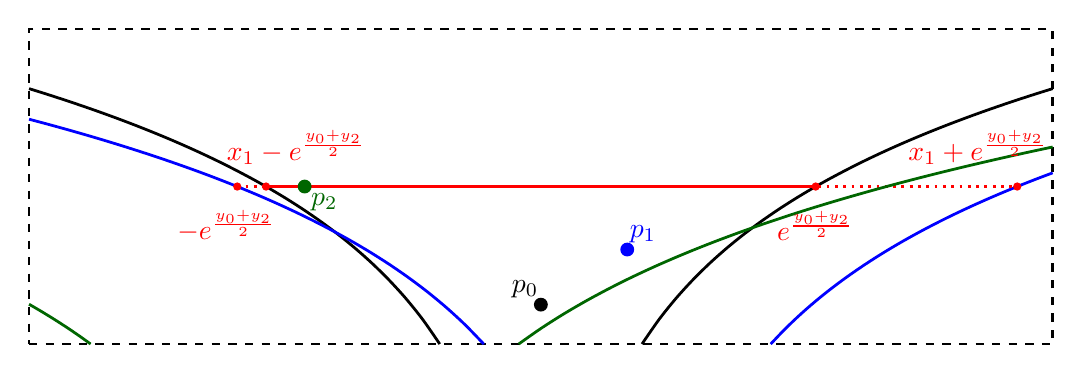
\begin{tikzpicture}
	%Define the coordinates 
	%p = (\u,\v) and p^\prime = (\uu, \vv)
	%Box \Rcal_n has width 2\r and height \t
	\pgfmathsetmacro{\u}{0} %0
	\pgfmathsetmacro{\v}{0.5} %1
	\pgfmathsetmacro{\vv}{1.2} %0.8
	\pgfmathsetmacro{\vvv}{2} %0.8
	\pgfmathsetmacro{\uuu}{-3} %1.4	
	\pgfmathsetmacro{\r}{6.5}
	\pgfmathsetmacro{\t}{4}
	
	\pgfmathsetmacro{\ubound}{exp((\vv+\vvv)/2)-exp((\v+\vvv)/2)}
	
	\pgfmathsetmacro{\uu}{3*\ubound/4}
	
	\pgfmathsetmacro{\leftintvandvvv}{-exp((\v + \vvv)/2)}
	\pgfmathsetmacro{\rightintvandvvv}{exp((\v + \vvv)/2)}
	\pgfmathsetmacro{\leftintvvandvvv}{\uu-exp((\vv + \vvv)/2)}
	\pgfmathsetmacro{\rightintvvandvvv}{\uu+exp((\vv + \vvv)/2)}
		
	%The box \Rcal_n
	\draw[line width=1pt,dashed] (-\r,0) -- (\r,0) -- (\r,\t) -- (-\r,\t) -- (-\r,0);

	%Dram all three nodes
    \draw node[fill, circle, inner sep=0pt, minimum size=5pt] (p1) at (\u,\v) {};
    \path (p1)+(-0.2,0.2) node {$p_0$};
    \draw node[fill,blue, circle, inner sep=0pt, minimum size=5pt] (p2) at (\uu,\vv) {};
    \path (p2)+(0.2,0.2) node {\color{blue}$p_1$};	
	
	%Boundaries p_0 = (\u,\v)
	
	%Right boundary
	\pgfmathsetmacro{\rightbounduv}{\u+exp((\v)/2)}
	\draw[domain=\rightbounduv:\r,smooth,variable=\x,black,line width=1pt] plot (\x, {2*ln(\x)-\v});
    %Left boundary
    \pgfmathsetmacro{\leftbounduv}{\u-exp((\v)/2)}
    \draw[domain=\leftbounduv:-\r,smooth,variable=\x,black,line width=1pt] plot (\x, {2*ln(-\x)-\v});
    
    %Boundaries p_1 = (\uu,\vv)
    
    %Right boundary
    \pgfmathsetmacro{\rightbounduuvv}{\uu+exp((\vv)/2)}
    \draw[domain=\rightbounduuvv:\r,smooth,variable=\x,blue,line width=1pt] plot (\x, {2*ln(\x-\uu)-\vv});
%    %Shifted right boundary
%    \pgfmathsetmacro{\shiftrightbounduuvv}{\uu+exp((\vv + \t)/2)-2*\r}
%    \draw[domain=\shiftrightbounduuvv:-\r,smooth,variable=\x,blue,line width=1pt] plot (\x, {2*ln(\x+(2*\r-\uu))-\vv});
    %Left boundary 
    \pgfmathsetmacro{\leftbounduuvv}{\uu-exp((\vv)/2)}
    \draw[domain=\leftbounduuvv:-\r,smooth,variable=\x,blue,line width=1pt] plot (\x, {2*ln(\uu-\x)-\vv});
%    %Shifted left boundary
%    \pgfmathsetmacro{\shiftleftbounduuvv}{\uu-exp((\vv + \t)/2)+2*\r}
%    \draw[domain=\shiftleftbounduuvv:\r,smooth,variable=\x,blue,line width=1pt] plot (\x, {2*ln(2*\r + \uu-\x)-\vv});
   


	\draw [red,dotted,line width=1pt] (\leftintvandvvv,\vvv) -- (\rightintvandvvv,\vvv);
	
	\draw [red,dotted,line width=1pt] (\leftintvvandvvv,\vvv) -- (\rightintvvandvvv,\vvv);

	\draw [red,line width=1pt] (\leftintvandvvv,\vvv) -- (\rightintvandvvv,\vvv);

    \draw node[fill,black!60!green, circle, inner sep=0pt, minimum size=5pt] (p2) at (\uuu,\vvv) {};
    \path (p2)+(0.25,-0.2) node {\color{black!60!green}$p_2$};
    
	%Boundaries p_2 = (\uuu,\vvv)
	
	%Right boundary
	\pgfmathsetmacro{\rightbounduuuvvv}{\uuu+exp((\vvv)/2)}
	\draw[domain=\rightbounduuuvvv:\r,smooth,variable=\x,black!60!green,line width=1pt] plot (\x, {2*ln(\x-\uuu)-\vvv});
    %Left boundary
    \pgfmathsetmacro{\leftbounduuuvvv}{\uuu-exp((\vvv)/2)}
    \draw[domain=\leftbounduuuvvv:-\r,smooth,variable=\x,black!60!green,line width=1pt] plot (\x, {2*ln(\uuu-\x)-\vvv});

	\draw node[fill,red, circle, inner sep=0pt, minimum size=3pt] at (\leftintvandvvv,\vvv) {};
	\path (\leftintvandvvv,\vvv)+(-0.5,-0.5) node[red] {$-e^{\frac{y_0 + y_2}{2}}$};
	\draw node[fill,red, circle, inner sep=0pt, minimum size=3pt] at (\rightintvandvvv,\vvv) {};
	\path (\rightintvandvvv,\vvv)+(0,-0.5) node[red] {$e^{\frac{y_0 + y_2}{2}}$};
	
	\draw node[fill,red, circle, inner sep=0pt, minimum size=3pt] at (\leftintvvandvvv,\vvv) {};
	\path (\leftintvvandvvv,\vvv)+(0.75,0.5) node[red] {$x_1 - e^{\frac{y_0 + y_2}{2}}$};
	\draw node[fill,red, circle, inner sep=0pt, minimum size=3pt] at (\rightintvvandvvv,\vvv) {};
	\path (\rightintvvandvvv,\vvv)+(-0.5,0.5) node[red] {$x_1 + e^{\frac{y_0 + y_2}{2}}$};

\end{tikzpicture}\\
\vspace{0.5cm}
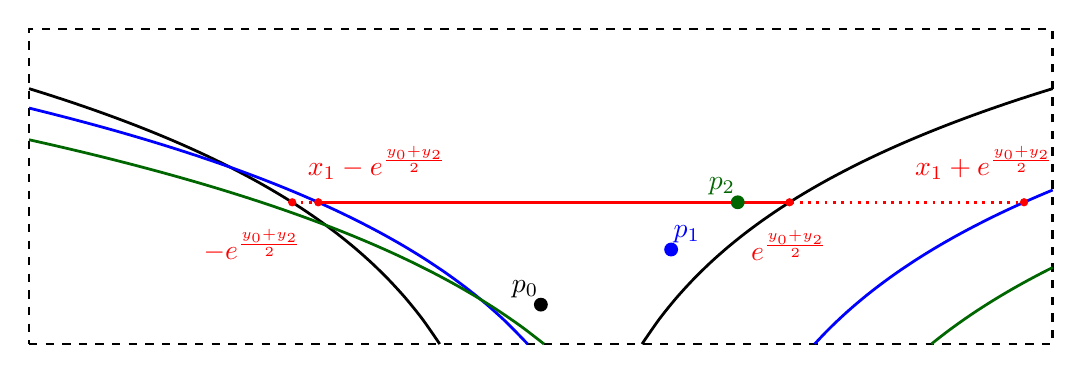
\begin{tikzpicture}
	%Define the coordinates 
	%p = (\u,\v) and p^\prime = (\uu, \vv)
	%Box \Rcal_n has width 2\r and height \t
	\pgfmathsetmacro{\u}{0} %0
	\pgfmathsetmacro{\v}{0.5} %1
	\pgfmathsetmacro{\vv}{1.2} %0.8
	\pgfmathsetmacro{\vvv}{1.8} %0.8
	\pgfmathsetmacro{\uuu}{2.5} %1.4	
	\pgfmathsetmacro{\r}{6.5}
	\pgfmathsetmacro{\t}{4}
	
	\pgfmathsetmacro{\ubound}{exp((\vv+\vvv)/2)-exp((\v+\vvv)/2)}
	
	\pgfmathsetmacro{\uu}{5*\ubound/4}
	
	\pgfmathsetmacro{\leftintvandvvv}{-exp((\v + \vvv)/2)}
	\pgfmathsetmacro{\rightintvandvvv}{exp((\v + \vvv)/2)}
	\pgfmathsetmacro{\leftintvvandvvv}{\uu-exp((\vv + \vvv)/2)}
	\pgfmathsetmacro{\rightintvvandvvv}{\uu+exp((\vv + \vvv)/2)}
		
	%The box \Rcal_n
	\draw[line width=1pt,dashed] (-\r,0) -- (\r,0) -- (\r,\t) -- (-\r,\t) -- (-\r,0);

	%Dram all three nodes
    \draw node[fill, circle, inner sep=0pt, minimum size=5pt] (p1) at (\u,\v) {};
    \path (p1)+(-0.2,0.2) node {$p_0$};
    \draw node[fill,blue, circle, inner sep=0pt, minimum size=5pt] (p2) at (\uu,\vv) {};
    \path (p2)+(0.2,0.2) node {\color{blue}$p_1$};	
	
	%Boundaries p_0 = (\u,\v)
	
	%Right boundary
	\pgfmathsetmacro{\rightbounduv}{\u+exp((\v)/2)}
	\draw[domain=\rightbounduv:\r,smooth,variable=\x,black,line width=1pt] plot (\x, {2*ln(\x)-\v});
    %Left boundary
    \pgfmathsetmacro{\leftbounduv}{\u-exp((\v)/2)}
    \draw[domain=\leftbounduv:-\r,smooth,variable=\x,black,line width=1pt] plot (\x, {2*ln(-\x)-\v});
    
    %Boundaries p_1 = (\uu,\vv)
    
    %Right boundary
    \pgfmathsetmacro{\rightbounduuvv}{\uu+exp((\vv)/2)}
    \draw[domain=\rightbounduuvv:\r,smooth,variable=\x,blue,line width=1pt] plot (\x, {2*ln(\x-\uu)-\vv});
    %Left boundary 
    \pgfmathsetmacro{\leftbounduuvv}{\uu-exp((\vv)/2)}
    \draw[domain=\leftbounduuvv:-\r,smooth,variable=\x,blue,line width=1pt] plot (\x, {2*ln(\uu-\x)-\vv});


	\draw [red,dotted,line width=1pt] (\leftintvandvvv,\vvv) -- (\rightintvandvvv,\vvv);
	
	\draw [red,dotted,line width=1pt] (\leftintvvandvvv,\vvv) -- (\rightintvvandvvv,\vvv);

	\draw [red,line width=1pt] (\leftintvvandvvv,\vvv) -- (\rightintvandvvv,\vvv);
	


    \draw node[fill,black!60!green, circle, inner sep=0pt, minimum size=5pt] (p2) at (\uuu,\vvv) {};
    \path (p2)+(-0.2,0.2) node {\color{black!60!green}$p_2$};
    
	%Boundaries p_2 = (\uuu,\vvv)
	
	%Right boundary
	\pgfmathsetmacro{\rightbounduuuvvv}{\uuu+exp((\vvv)/2)}
	\draw[domain=\rightbounduuuvvv:\r,smooth,variable=\x,black!60!green,line width=1pt] plot (\x, {2*ln(\x-\uuu)-\vvv});
    %Left boundary
    \pgfmathsetmacro{\leftbounduuuvvv}{\uuu-exp((\vvv)/2)}
    \draw[domain=\leftbounduuuvvv:-\r,smooth,variable=\x,black!60!green,line width=1pt] plot (\x, {2*ln(\uuu-\x)-\vvv});

	\draw node[fill,red, circle, inner sep=0pt, minimum size=3pt] at (\leftintvandvvv,\vvv) {};
	\path (\leftintvandvvv,\vvv)+(-0.5,-0.55) node[red] {$-e^{\frac{y_0 + y_2}{2}}$};
	\draw node[fill,red, circle, inner sep=0pt, minimum size=3pt] at (\rightintvandvvv,\vvv) {};
	\path (\rightintvandvvv,\vvv)+(0,-0.55) node[red] {$e^{\frac{y_0 + y_2}{2}}$};
	
	\draw node[fill,red, circle, inner sep=0pt, minimum size=3pt] at (\leftintvvandvvv,\vvv) {};
	\path (\leftintvvandvvv,\vvv)+(0.75,0.5) node[red] {$x_1 - e^{\frac{y_0 + y_2}{2}}$};
	\draw node[fill,red, circle, inner sep=0pt, minimum size=3pt] at (\rightintvvandvvv,\vvv) {};
	\path (\rightintvvandvvv,\vvv)+(-0.5,0.5) node[red] {$x_1 + e^{\frac{y_0 + y_2}{2}}$};

\end{tikzpicture}
\caption{Situation for the intersections of the connection intervals considered in Lemma~\ref{lem:ordered}, with $y_0 < y_1 <y_2$ fixed and for different cases of $0 \le x_1 \le e^{(y_0 + y_1)/2}$. The top figure shows the case where $0 \le x_1 \le e^{(y_1 + y_2)/2} - e^{(y_0 + y_2)/2}$, while the bottom one shows the case $x_1 > e^{(y_1 + y_2)/2} - e^{(y_0 + y_2)/2}$. The solid red line indicates the range for $x_2$ such that the points $p_0$, $p_1$ and $p_2$ form a triangle. The boundaries of there balls are show in, respectively, black, blue and green.}
\label{fig:triangle_prob_lemma}
\end{figure}

\begin{proof}
%pim pass1: $P(y_0,y_1,y_2)$ is the probability that $(x_1,y_1)$ and $(x_2,y_2)$ (which are given by a Poisson process in the upper half-plane) are neighbours of each other, given that they are neighbours of $(0,y_0)$ (see figure \ref{fig:triangle_prob_lemma}). By the properties of the Poisson process and our connection rule (which defines the neighourhood area of $(0,y_0)$ in the upper half-plane), given $y_0, y_1, y_2$ we have that $x_i$ is chosen u.a.r.~from $[-e^{y_0/2+y_i/2}, +e^{y_0/2+y_i/2}]$ for $i=1,2$.
Since the Poisson Point Process is translation invariant in the $x$-coordinate we can, without loss of generality, take $x_0 = 0$. By definition of the connection rule $P(y_0,y_1,y_2)$ is the probability that $|x_2-x_1| \leq  e^{(y_1+y_2)/2}$ (see figure \ref{fig:triangle_prob_lemma}). Consider $y_0, y_1, y_2$ and $x_1$ fixed. Then we are interested in computing the probability that $x_2$ falls into the interval $[x_1-e^{(y_1+y+2)/2},x_1+e^{(y_1+y_2)/2}]$ (given by the bottom interval in the Figure~\ref{fig:triangle_prob_lemma}), as well as into the interval $[-e^{(y_0+y_2)/2},e^{(y_0+y_2)/2}]$ (given by the top interval in the Figure~\ref{fig:triangle_prob_lemma}).

%, i.e. the desired probability can be written as
%\[ 
%\frac{
%\Ee_{x_1} \text{length}( [x_1-e^{(y_1+y_2)/2}, x_1+e^{(y_1+y_2)/2}] \cap [-e^{(y_0+y_2)/2}, e^{(y_0+y_2)/2}] )
%}{
%2 e^{(y_0+y_2)/2}
%} \]
%
%\noindent

By symmetry, without loss of generality we can consider $x_1$ uniformly at random from $[0,e^{y_0/2+y_1/2}]$. 
%The probability will be the same.Let us assume for the moment that $y_0 < y_1 < y_2$. 
Since $y_0 < y_1 < y_2$ we have that $e^{(y_1+y_2)/2} > e^{(y_0+y_2)/2}$ and so, when $x_1 \geq 0$, the ``right half'' of the interval $[-e^{(y_0+y_2)/2}, e^{(y_0+y_2)/2}]$ is always covered by the interval $[x_1-e^{(y_1+y_2)/2}, x_1+e^{(y_1+y_2)/2}]$.
If $e^{(y_1+y_2)/2} - e^{(y_0+y_1)/2} \geq e^{(y_0+y_2)/2}$ then the ``left half'' is always covered as well.
In other words:
\[
	e^{(y_1+y_2)/2} - e^{(y_0+y_1)/2} \geq e^{(y_0+y_2)/2} \Rightarrow P(y_0,y_1,y_2) = 1.
\]

Now consider the case where $e^{(y_1+y_2)/2} - e^{(y_0+y_1)/2} < e^{(y_0+y_2)/2}$. Then, if $x_1 \in [0, e^{(y_1+y_2)/2} - e^{(y_0+y_2)/2}]$ the whole interval $[-e^{(y_0+y_2)/2}, e^{(y_0+y_2)/2}]$ is still covered so that $p_0, p_1$ and $p_2$ form a triangle. If, on the other hand $e^{(y_1+y_2)/2} - e^{(y_0+y_2)/2} < x_1 \leq e^{(y_0+y_1)/2}$ then
the probability that $|x_2-x_1| \leq e^{(y_1+y_2)/2}$ equals
\[ 
	1 - \frac{x_1 - (e^{(y_1+y_2)/2} - e^{(y_0+y_2)/2)}) }{ 2e^{(y_0+y_2)/2} }. 
\]

Hence, when $e^{(y_1+y_2)/2} - e^{(y_0+y_1)/2} < e^{(y_0+y_2)/2}$ we have
\begin{align*}
	P(y_0,y_1,y_2) &= \frac{e^{(y_1+y_2)/2} - e^{(y_0+y_2)/2} }{ e^{(y_0+y_1)/2} }  \\
	&\hspace{10pt}+ \int_{ e^{(y_1+y_2)/2} - e^{(y_0+y_2)/2} }^{ e^{(y_0+y_1)/2} } 
	    \left(1 - \frac{x_1 - (e^{(y_1+y_2)/2} - e^{(y_0+y_2)/2)}) }{ 2e^{(y_0+y_2)/2} }\right)
	    \cdot \frac{1}{e^{(y_0+y_1)/2}} \dd x_1 \\
	&= 1 - \frac{1}{2e^{y_0+y_1/2+y_2/2} } \int_0^{ e^{(y_0+y_1)/2}+e^{(y_0+y_2)/2}-e^{(y_1+y_2)/2} } x_1 \dd x_1 \\
	&= 1 - \frac{ \left( e^{(y_0+y_1)/2}+e^{(y_0+y_2)/2}-e^{(y_1+y_2)/2} \right)^2 }{ 4 e^{y_0+y_1/2+y_2/2} },
\end{align*}

At this point it is convenient to rewrite everything in terms of $z_i := e^{-y_i/2}$.
Note that $y_0 < y_1 < y_2$ if and only if $z_0 > z_1 > z_2$ while the condition $e^{(y_1+y_2)/2} - e^{(y_0+y_1)/2} < e^{(y_0+y_2)/2}$ becomes
\[ e^{(y_1+y_2)/2} - e^{(y_0+y_1)/2} < e^{(y_0+y_2)/2} \Leftrightarrow 
z_1^{-1} z_2^{-1} < z_0^{-1} z_1^{-1} + z_0^{-1}z_2^{-1} 
\Leftrightarrow
z_0 < z_1+z_2. 
\]

We now conclude that
\[
	P(y_0(z_0), y_1(z_1), y_2(z_2)) = 1 \quad \text{if} \quad z_0 > z_1 > z_2 \text{ and } z_0 \geq z_1 + z_2
\]
while for $z_0 > z_1 > z_2$ and $z_0 < z_1 + z_2$
\begin{align*}
	P(y_0, y_1, y_2) 
	&= 1 - \frac{z_0^2z_1z_2}{4} \cdot \left( z_0^{-1}z_1^{-1}+z_0^{-1}z_2^{-1}-z_1^{-1}z_2^{-1} \right)^2 \\
%	&= 1 - \frac{z_0^2z_1z_2}{4} \cdot \left( z_0^{-2}z_1^{-2} + z_0^{-2}z_2^{-2} + z_1^{-2}z_2^{-2}
%		+ 2z_0^{-2}z_1^{-1}z_2^{-1} - 2 z_0^{-1}z_1^{-2}z_2^{-1} - 2z_0^{-1}z_1^{-1}z_2^{-2} \right) \\
	&= 1 - \frac{1}{4} \left( z_1^{-1}z_2 + z_1z_2^{-1} + z_0^2z_1^{-1}z_2^{-1} + 2 - 2z_0z_1^{-1}-2z_0z_2^{-1}\right),
\end{align*}
which finishes the proof.
\end{proof}

The previous lemma covers the case when $y_0<y_1<y_2$. We now leverage it to take care of the other cases as well. 

\begin{proof}[Proof of Lemma~\ref{lem:triangle_prob_y_coordinates}]
Let $y_i >0$ and $z_i = e^{-y_i/2}$, $i=0,1,2$. Lemma~\ref{lem:ordered} gives the expression for $P(y_0(z_0),y_1(z_1),y_2(z_2))$ in the case $y_0<y_1<y_2$, or equivalently $z_0>z_1>z_2$, i.e. the first two lines in the claim of Lemma~\ref{lem:triangle_prob_y_coordinates}. To analyze the other cases we shall express $P(y_1,y_0,y_2)$ and $P(y_1,y_2,y_0)$ in terms of $P(y_0,y_1,y_2)$ and $z_i$. For this we note that we can view $P(y_0,y_1,y_2)$ as a 2-fold integral of the indicator function
\[ 
	h(x_0, x_1, x_2) := \ind{ |x_0 - x_1| < e^{(y_0+y_1)/2}, |x_0 - x_2| < e^{(y_0+y_2)/2}, |x_1-x_2| < e^{(y_1+y_2)/2}}, 
\]
where $x_0$ was set to zero, without loss of generality, and the other two $x_i$ are uniform random variables on $[-e^{(y_0)+y_i)/2}, e^{(y_0+y_i)/2}]$. When we consider the probability $P(y_1,y_0,y_2)$, this is the 2-fold integral of $h(x_0,0,x_2)$ so that
\begin{align*}
	P(y_1,y_0,y_2) &= \frac{1}{2e^{(y_1+y_0)/2}} \cdot \frac{1}{2e^{(y_1+y_2)/2}} 
		\iint_{\R} h(x_0,0,x_2) \dd x_0 \dd x_2\\
	&= \frac{e^{y_0/2}}{e^{y_1/2}} \frac{1}{2e^{(y_0+y_1)/2}} \frac{1}{2e^{(y_0+y_2)/2}} 
		\iint_{\R} h(0,x_1,x_2) \dd x_1 \dd x_2\\
	&= \frac{e^{y_0/2}}{e^{y_1/2}} P(y_0,y_1,y_2) = \frac{z_1}{z_0}  P(y_0,y_1,y_2).
\end{align*}
Finally we note that $h(x_0,0,x_2) = h(x_2,0,x_0)$ from which we conclude that
\begin{equation}\label{eq:symmetry_relation_triangle_prob}
	P(y_0, y_1, y_2) = \left(z_0/z_1\right) P(y_1,y_0,y_2) = \left(z_0/z_1\right) P(y_1,y_2,y_0).
\end{equation}

To complete the proof for the other cases we note that since $P(y_0,y_1,y_2)$ is symmetric in $y_1$ and $y_2$, we can assume, without loss of generality, that $y_1 < y_2$. Then, there are two more orderings of $y_0, y_1, y_2$, namely $y_1< y_0< y_2$ and $y_1<y_2<y_0$, which can be summarized as $y_1 < \min (y_0,y_2)$, or equivalently $z_1 > \max(z_0,z_2)$. For $y_1 < y_0 < y_2$ and $y_1 < y_2<y_0$ we can apply Lemma~\ref{lem:ordered} to obtain $P(y_1,y_0,y_2) = P(y_1,y_2,y_0)$ which happen to agree due to the symmetry in the last two arguments of the expression found in Lemma~\ref{lem:ordered}. The expression for $P(y_0,y_1,y_2)$ then follows from~\eqref{eq:symmetry_relation_triangle_prob}.
\end{proof}

%\begin{lemma}\label{lem:leverage}
%We have
%
%\[ P(y_0, y_1, y_2) = \left(z_0/z_1\right) P(y_1,y_0,y_2) = \left(z_0/z_1\right) P(y_1,y_2,y_0), \]
%
%\noindent
%where $z_i = e^{-y_i/2}$ as before.
%\end{lemma}
%
%
%
%\begin{proof}
%We can think of $P(y_0,y_1,y_2)$ as a multiple of a 3-fold integral of the indicator function
%\[ 
%	h(x_0, x_1, x_2) := \ind{ |x_0-x_1| < e^{(y_0+y_1)/2}, |x_0-x_2| < e^{(y_0+y_2)/2}, |x_1-x_2| < e^{(y_1+y_2)/2}}, 
%\]
%where $x_0$ is selected uniformly $ x_1, x_2$ range over $\R$. More specifically $x_0$ u.a.r.~from $[-K,+K]$ and $x_i$ u.a.r.~from 
%$[x_0-e^{(y_0+y_i)/2}, x_0+e^{(y_0+y_i)/2}]$
%
%which we make into a 
%circle by identifying the endpoints and we take $K$ large enough.
%In more detail: we integrate the indicator function 
%
%\[ 
%	h(x_0, x_1, x_2) := 1_{\{ |x_0-x_1|_{2K} < e^{(y_0+y_1)/2}, |x_0-x_2|_{2K} < e^{(y_0+y_2)/2}, |x_1-x_2|_{2K} < e^{(y_1+y_2)/2} \}}, 
%\]
% 
%(where $|a|_b := \min(|a|, b-|a|)$ for $|a| \leq b$), and we multiply by 
%$\frac{1}{2K} \cdot \frac{1}{2e^{(y_0+y_1)/2}} \cdot \frac{1}{2e^{(y_0+y_2)/2}}$.
%(we think of taking $x_0$ u.a.r.~from $[-K,+K]$ and $x_i$ u.a.r.~from 
%$[x_0-e^{(y_0+y_i)/2}, x_0+e^{(y_0+y_i)/2}]$ -- interpreted modulo $K$ of course, so $K$ is chosen as a real number $>e^{(y_0+y_i)/2}$  s.t. the intervals $[x_0-e^{(y_0+y_i)/2},x_0+e^{(y_0+y_i)/2}]$ do not cover the circle).
%That is:
%
%\[ P(y_0, y_1, y_2) = \frac{1}{2K} \cdot \frac{1}{2e^{(y_0+y_1)/2}} \cdot \frac{1}{2e^{(y_0+y_2)/2}} \cdot \int_{[-K,K]^3} f. \]
%
%\noindent
%Completely analogously:
%
%\[ P(y_1,y_0,y_2) = \frac{1}{2K} \cdot \frac{1}{2e^{(y_1+y_0)/2}} \cdot \frac{1}{2e^{(y_1+y_2)/2}} \cdot \int_{[-K,K]^3} f
% = \frac{e^{y_0/2}}{e^{y_1/2}} P(y_0,y_1,y_2) = \frac{z_1}{z_0}  P(y_0,y_1,y_2), \]
%
%\noindent
%proving the first part of the lemma. The second part of the lemma holds as $P(y_1,y_2,y_0)=P(y_1,y_0,y_2)$.
%\end{proof}
%
%\begin{corollary} \label{cor:nonordered}
%$\text{ }$
%If $y_1 < \min(y_0,y_2)$ (or equivalently $z_1 > \max(z_0,z_2)$), then 
%\[ P(y_0,y_1,y_2) = \left\{ 
%\begin{array}{cl}
%\frac{z_0}{z_1} & \text{ if } z_1 \geq z_0 + z_2, \\
%\frac{z_0}{z_1} \cdot (1-G(z_1,z_0,z_2)) & \text{ if } z_1 < z_0+z_2. 
%\end{array} \right. 
%\]
%
%(Here $z_i := e^{-y_i/2}$ as before.)
%\end{corollary}
%
%Applying the expression found earlier, we find that 
%
%\[ \begin{array}{rcl}
%G(z_1,z_0,z_2)
%& = & 
%\frac14 ( z_0^{-1} z_2 + z_0 z_2^{-1} + z_1^2z_0^{-1} z_2^{-1}
%+ 2 -2z_1z_0^{-1}-2z_1z_2^{-1} ) \\
%\end{array} \]
%
%%\noindent
%Hence
%
%\[ \begin{array}{rcl}
%    G'(z_0,z_1,z_2) 
%    & := &  \frac{z_0}{z_1} G(z_1,z_0,z_2) \\
%    & = & \frac14 ( z_1^{-1} z_2 +z_0^2 z_1^{-1} z_2^{-1} + z_1 z_2^{-1} + 2z_0z_1^{-1} - 2 - 2z_0z_2^{-1} )
%   \end{array}
%\]
%
%We are now ready to complete the proof of Lemma~\ref{lem:triangle_prob_y_coordinates}.
%
%\begin{proof}[Proof of Lemma~\ref{lem:triangle_prob_y_coordinates}]
%Let $y_i >0$ and $z_i = e^{-y_i/2}$, $i=0,1,2$. Then lemma \ref{lem:ordered} gives the expression for $P(y_0(z_0),y_1(z_1),y_2(z_2))$ in the case $y_0<y_1<y_2$, or equivalently $z_0>z_1>z_2$, i.e. the first two lines in the claim of the proposition. As $P(y_0,y_1,y_2)$ is symmetric in $y_1$ and $y_2$, we can assume $y_1 < y_2$. Then, there are two more orderings of $y_0, y_1, y_2$, namely $y_1< y_0< y_2$ and $y_1<y_2<y_0$. That either of these orderings holds is equivalent to $y_1 < \min (y_0,y_2)$, or equivalently to $z_1 > \max(z_0,z_2)$. For $y_1 < y_0 < y_2$ and $y_1 < y_2<y_0$ we can apply lemma \ref{lem:ordered} to obtain $P(y_1,y_0,y_2)$ and $P(y_1,y_2,y_0)$ which happen to agree due to the symmetry in the last two arguments of the expression found in that lemma. Then lemma \ref{lem:leverage} yields $P(y_0,y_1,y_2)$ based on $P(y_1,y_0,y_2)=P(y_1,y_2,y_0)$ and corollary \ref{cor:nonordered} spells this out explicitly and together with the remarks after corollary \ref{cor:nonordered}, we obtain the remaining two lines in the claim of the proposition, which concludes the proof.
%\end{proof}

\subsection{Computing $\Delta_\Pcal(y_0)$}

Now that we have established the expression for $P(y_0,y_1,y_2)$ we can proceed with computing $\Delta_{\Pcal}(y_0)$, i.e. proving Proposition~\ref{prop:full_expression_delta_P}. We start with the following observation.

\begin{lemma}\label{lem:continuity_Delta_function}
The function $\alpha \mapsto \Delta_{\Pcal_{\alpha,\nu}}(y_0)$ is continuous for all $\alpha > \frac{1}{2}$.
\end{lemma}
\begin{proof}
This follows from the theorem of dominated convergence:
Let $\alpha > \frac{1}{2}$ and $(\alpha_n)_{n\in \mathbb{N}}$ a sequence of real numbers converging to $\alpha$, so we can assume $|\alpha_n - \alpha| < \epsilon := \frac{\alpha-1/2}{2}$. This means that $-\epsilon < \alpha_n - \alpha < \epsilon$, i.e. $\frac{\alpha-1/2}{2} < \alpha_n - 1/2 < \frac{3\alpha-3/2}{2}$. Define $f_n(y_1,y_2) = P(y_0,y_1,y_2) (\alpha_n - 1/2)^2 e^{-(\alpha_n-1/2)(y_1+y_2)}$. As the function $x \mapsto x^2$ is increasing in $x$ for $x>0$ and the function $x \mapsto e^{-(y_1+y_2)x}$ is decreasing in $x$ and $P(y_0,y_1,y_2) \in [0,1]$, it holds that $|f_n(y_1,y_2)| \leq (\frac{3\alpha-3/2}{2})^2e^{-(y_1+y_2)\frac{\alpha-1/2}{2}}$ which is integrable over $\R_{\geq 0} \times \R_{\geq 0}$ (with integral equals $\frac{(6\alpha-3)^2}{(2\alpha-1)^2}$). Application of the theorem of dominated convergence and using equation~\eqref{eq:def_delta_p} yields that $\Delta_{\Pcal_{\alpha_n,\nu}}(y_0) \rightarrow \Delta_{\Pcal_{\alpha,\nu}}(y_0)$ which gives the claim as the sequence $(\alpha_n)_n$ was arbitrary.
\end{proof}

Due to this lemma we can first assume $\alpha \notin \{ \frac{3}{4},1 \}$, compute $\Delta_{\Pcal}(y_0)$ and then obtain the values of $\Delta_\Pcal(y_0)$ at the remaining two points by taking the corresponding limit in $\alpha$. This strategy is executed below. It involves the computation of several integrals which are involved and will take up the next 7 pages. The proof is carefully structured, using headers, to aid the reader. 

\begin{proof}[Proof of Proposition~\ref{prop:full_expression_delta_P}]\hfill

\paragraph{When $\bm{\alpha \notin \{3/4,1\}}$}
Note that when writing $\Delta_{\Pcal}(y_0)$ as in integral as in equation \eqref{eq:def_delta_p}, by symmetry in the integration variables $y_1$ and $y_2$, we can assume that $y_1<y_2$ in which case either $y_0$ or $y_1$ is the smallest height. This gives half the value of $\Delta_{\Pcal}(y_0)$ and hence
\[ 
	\Delta_\Pcal(y_0) = 2(I_1(y_0) +I_2(y_0)), 
\] 
where $I_1$ and $I_2$ are given by:
\begin{align*}
	I_1(y_0) &:= \int_{0<y_0<y_1<y_2} P(y_0,y_1,y_2) \cdot (\alpha-1/2)^2 e^{-(\alpha-1/2)(y_1+y_2)}  {\dd} y_2 {\dd} y_1 \\ 
	I_2(y_0) &:= \int_{0<y_1<y_0,y_2} P(y_0,y_1,y_2) \cdot (\alpha-1/2)^2 e^{-(\alpha-1/2)(y_1+y_2)} {\dd} y_2 {\dd} y_1 \\ 
\end{align*}

We proceed with computing each of these two integrals, each of which is split in two parts. The final expressions of those four integrals can be found in~\eqref{eq:Delta_P_computation_I11}, \eqref{eq:Delta_P_computation_I12}, \eqref{eq:Delta_P_computation_I21} and~\eqref{eq:Delta_P_computation_I22}.

\paragraph{Computing $\bm{I_1(y_0)}$}

Applying the change of variables $z_i := e^{-y_i/2}$ and Lemma~\ref{lem:triangle_prob_y_coordinates} gives %${\dd}y_i = -\frac{2{\dd}z_i}{z_i}$ and therefore
\begin{align*}
	I_1(y_0) &=	4 (\alpha-1/2)^2 \cdot \int_{z_0>z_1>z_2>0} P(y_0,y_1(z),y_2(z)) z_1^{2\alpha-2} z_2^{2\alpha-2} 
		{\dd}z_2{\dd}z_1 \\
	&= 4 (\alpha-1/2)^2 \cdot \left( \int_{z_0>z_1>z_2>0} 1 \cdot z_1^{2\alpha-2} z_2^{2\alpha-2} 
		{\dd}z_2{\dd}z_1 \right. \\
	&\hspace{10pt} \left. - \int_{{z_0>z_1>z_2>0,}\atop{z_0 < z_1+z_2}} G(z_0,z_1,z_2) \cdot z_1^{2\alpha-2} z_2^{2\alpha-2} 
		{\dd}z_2{\dd}z_1 \right) \\
	&=: 4 (\alpha-1/2)^2 ( I_{11}(y_0) - I_{12}(y_0)). \numberthis \label{eq:Delta_P_computation_I11}
\end{align*}

The integral $I_{11}(y_0)$ is easily obtained:
\begin{align*}
	I_{11}(y_0) &= \int_0^{z_0} \int_0^{z_1} z_1^{2\alpha-2} z_2^{2\alpha-2} {\dd}z_2{\dd}z_1\\
	&= \int_0^{z_0} z_1^{2\alpha-2} \left[ \frac{z_2^{2\alpha-1}}{2\alpha-1} \right]_0^{z_1} {\dd}z_1\\
	&= \frac{1}{2\alpha-1} \cdot \int_0^{z_0} z_1^{4\alpha-3} {\dd}z_1 \\
	&= \frac{1}{2(2\alpha-1)^2} \cdot z_0^{4\alpha-2}.
\end{align*}

To deal with $I_{12}$ we note that $G(z_0,z_1,z_2)$ is a linear combination of monomials of the form $z_0^az_1^bz_2^c$ with 
$a,b,c \in \{-1,0,1,2\}$ and $a+b+c=0$. Let us consider the integral $J_(a,b,c)(z_0)$
\begin{equation}\label{eq:def_Delta_P_computation_int_J_1}
	J_{a,b,c}(z_0) := z_0^a \int_{{z_0>z_1>z_2>0,}\atop{z_0 < z_1+z_2}} z_1^{b+2\alpha-2} z_2^{c+2\alpha-2} {\dd}z_2{\dd}z_1.
\end{equation}
and note that
\begin{equation}\label{eq:Delta_P_computation_I12_with_J}
	I_{1,2}(y_0) = \frac{1}{4} (J_{0,-1,1}(z_0)+J_{0,1,-1}(z_0)+J_{2,-1,-1}(z_0)+2J_{0,0,0}(z_0)-2J_{1,-1,0}(z_0)-2J_{1,0,-1}(z_0)).
\end{equation}

Next we compute $J_{a,b,c}(z_0)$.
\begin{align*}
	J_{a,b,c} 
	&= z_0^a \int_{z_0/2}^{z_0}\int_{z_0-z_1}^{z_1} z_1^{b+2\alpha-2} z_2^{c+2\alpha-2} {\dd}z_2{\dd}z_1
		= z_0^a \int_{z_0/2}^{z_0} z_1^{b+2\alpha-2} \left[ \frac{ z_2^{c+2\alpha-1} }{ c+2\alpha-1 } \right]_{z_0-z_1}^{z_1} \dd z_1\\
	&= \frac{z_0^a}{c+2\alpha-1} \cdot \left( \int_{z_0/2}^{z_0} z_1^{b+c+4\alpha-3} \dd z_1
	   - \int_{z_0/2}^{z_0} z_1^{b+2\alpha-2} (z_0-z_1)^{c+2\alpha-1} {\dd}z_1 \right) \\
	&= \frac{z_0^{a+b+c+4\alpha-2}(1-(1/2)^{b+c+4\alpha-2})}{(c+2\alpha-1)(b+c+4\alpha-2)} \\
	&\hspace{10pt}- \frac{z_0^{a+b+c+4\alpha-3}}{c+2\alpha-1} \int_{z_0/2}^{z_0}  \left(z_1/z_0\right)^{b+2\alpha-2} 
	    \left(1-(z_1/z_0)\right)^{c+2\alpha-1} \dd z_1\\
	&= \frac{z_0^{4\alpha-2}(1-(1/2)^{b+c+4\alpha-2})}{(c+2\alpha-1)(b+c+4\alpha-2)} 
		- \frac{z_0^{4\alpha-2}}{c+2\alpha-1}
	   \int_{1/2}^1  u^{b+2\alpha-2}(1-u)^{c+2\alpha-1} \dd u \\
	&= \frac{z_0^{4\alpha-2}(1-(1/2)^{b+c+4\alpha-2})}{(c+2\alpha-1)(b+c+4\alpha-2)} 
		- \frac{z_0^{4\alpha-2}}{c+2\alpha-1} B^-(1/2;c+2\alpha, b+2\alpha-1),
\end{align*}
where we've used the substitution $u := z_1/z_0$ giving $z_0 {\dd} u = {\dd} z_1$ in the penultimate line and
$B^-$ denotes the (lower) incomplete beta-function. Note that since $c \geq -1$, $-a \in \{0,-1,-2\}$ and by our assumption $\alpha \not \in \{\frac{3}{4}\}$, the denominators that occur during the integration are all non-zero.

Plugging this back into~\eqref{eq:Delta_P_computation_I12_with_J} gives
\begin{align*}
	I_{1,2}(y_0)
	&= \frac{z_0^{4\alpha-2}(1-(1/2)^{4\alpha-2})}{32\alpha(\alpha-1/2)} 
   		- \frac{z_0^{4\alpha-2}}{8\alpha} B^-(1/2;1+2\alpha, 2\alpha-2)\\
	&\hspace{10pt}+ \frac{z_0^{4\alpha-2}(1-(1/2)^{4\alpha-2})}{32(\alpha-1)(\alpha-1/2)} 
   		-  \frac{z_0^{4\alpha-2}}{4(2\alpha-2)} B^-(1/2;2\alpha-1,2\alpha)\\
	&\hspace{10pt}+ \frac{z_0^{4\alpha-2}(1-(1/2)^{4\alpha-4})}{32(\alpha-1)^2} 
   		- \frac{z_0^{4\alpha-2}}{4(2\alpha-2)} B^-(1/2;-1+2\alpha, 2\alpha-2)\\
	&\hspace{10pt}+ \frac{z_0^{4\alpha-2}(1-(1/2)^{4\alpha-2})}{16(\alpha-1/2)^2} 
   		- \frac{z_0^{4\alpha-2}}{2(2\alpha-1)} B^-(1/2;2\alpha,2\alpha-1)\\
	&\hspace{10pt}- \frac{z_0^{4\alpha-2}(1-(1/2)^{4\alpha-3})}{16(\alpha-1/2)(\alpha-3/4)} 
   		+ \frac{z_0^{4\alpha-2}}{2(2\alpha-1)} B^-(1/2;2\alpha, 2\alpha-2)\\
	&\hspace{10pt}- \frac{z_0^{4\alpha-2}(1-(1/2)^{4\alpha-3})}{16(\alpha-1)(\alpha-3/4)} 
   		+ \frac{z_0^{4\alpha-2}}{2(2\alpha-2)} B^-(1/2;-1+2\alpha, 2\alpha-1) \\
	&=\frac{\left(\frac{3}{64}- \frac{3}{16} 2^{-4\alpha}+ 
   		\alpha (-\frac{41}{128} + \frac{13}{16}  2^{-4\alpha}) 
   		+ \alpha^2 (\frac{5}{8} - \frac{3}{4} 2^{-4\alpha}) - \frac{15}{32}\alpha^3 +\frac{1}{8} a^4\right) 
   		z_0^{4 \alpha-2} }{4(\alpha-1/2)^2 (\alpha-1)^2 (\alpha-3/4) \alpha} \\
	&\hspace{10pt}+ \frac{z_0^{4\alpha-2}}{8 (\alpha-1) \alpha (2\alpha-1)}(4 (\alpha-1) \alpha 
		(B^-(1/2; 2\alpha, 2\alpha-2) - B^-(1/2;2 \alpha,2\alpha-1) ) \\
    &\hspace{10pt}- (2 \alpha-1)\alpha ( B^-(1/2; 2\alpha-1, 2\alpha-2) + 
    	B^-(1/2; 2\alpha-1, 2\alpha) - 
    	2 B^-(1/2;2\alpha -1, 2\alpha-1) ) \\
    &\hspace{10pt}- (2\alpha-1)(\alpha-1) B^-(1/2; 1 + 2\alpha, 2\alpha-2)) \\
	&=\frac{\left(\frac{3}{64}- \frac{3}{16} 2^{-4\alpha} 
		+ \alpha (-\frac{41}{128} + \frac{13}{16}  2^{-4\alpha})  
		+ \alpha^2 (\frac{5}{8} - \frac{3}{4} 2^{-4\alpha}) - \frac{15}{32}\alpha^3 +\frac{1}{8} a^4\right) 
		z_0^{4 \alpha-2} }{4(\alpha-1/2)^2 (\alpha-1)^2 (\alpha-3/4) \alpha} \\
 	&\hspace{10pt}+ \frac{z_0^{4\alpha-2}}{8 (\alpha-1) \alpha (2\alpha-1)}(4 (\alpha-1) \alpha 
 		B^-(1/2; 2\alpha+1, 2\alpha-2) \\
  	&\hspace{10pt}- (2 \alpha-1)\alpha B^-(1/2;2\alpha+1,2\alpha-2) \\
    &\hspace{10pt}- (2\alpha-1)(\alpha-1) B^-(1/2; 2\alpha+1, 2\alpha-2)). \\
\end{align*}
For the last step we use the identities 
\begin{align}
	B^-(z;a,b)-B^-(z;a,b+1) &= B^-(z; a+1,b), \label{eq:Delta_P_computation_beta_id_1}\\
	B^-(z;a,b)+B^-(z;a,b+2)-2B^-(z;a,b+1) &= B^-(z;a+2,b). \label{eq:Delta_P_computation_beta_id_2}
\end{align}
to obtain
\begin{equation}
\begin{aligned}
	I_{1,2}(y_0) &=\frac{\left(\frac{3}{64}- \frac{3}{16} 2^{-4\alpha}
		+ \alpha (-\frac{41}{128} + \frac{13}{16}  2^{-4\alpha})
		+ \alpha^2 (\frac{5}{8} - \frac{3}{4} 2^{-4\alpha}) - \frac{15}{32}\alpha^3 +\frac{1}{8} a^4\right) 
		z_0^{4 \alpha-2} }{4(\alpha-1/2)^2 (\alpha-1)^2 (\alpha-3/4) \alpha} \\
 	&\hspace{10pt}- \frac{z_0^{4\alpha-2}B^-(1/2; 2\alpha+1, 2\alpha-2) }{8 (\alpha-1) \alpha (2\alpha-1)}	\label{eq:Delta_P_computation_I12}
\end{aligned}
\end{equation}


\paragraph{Computing $\bm{I_2(y_0)}$}

We will follow a similar strategy as for $I_1(y_0)$. First, using the change of variables $z_i := e^{-y_i/2}$ and Lemma~\ref{lem:triangle_prob_y_coordinates} we get
\begin{align*}
	I_2(y_0) &= 4 (\alpha-1/2)^2 \cdot \int_{1>z_1>z_2,z_0>0} P(y_0(z_0),y_1(z_1),y_2(z_2)) z_1^{2\alpha-2} z_2^{2\alpha-2} 
		{\dd}z_2{\dd}z_1 \\
	&= 4 (\alpha-1/2)^2 \cdot \left( \int_{1>z_1>z_0,z_2>0}  z_0 z_1^{2\alpha-3} z_2^{2\alpha-2} 
		{\dd}z_2{\dd}z_1 \right. \\
	&\hspace{10pt}\left. - \int_{{1>z_1>z_0,z_2>0}\atop{z_1 < z_0+z_2}} G(z_1,z_0,z_2) z_0 z_1^{2\alpha-3} 	
		z_2^{2\alpha-2} \dd z_2{\dd}z_1 \right) \\
	&=: 4 (\alpha-1/2)^2 (I_{21}(y_0) - I_{22}(y_0)). \numberthis \label{eq:Delta_P_computation_I21}
\end{align*}

We proceed with the easy integral:
\begin{align*}
	I_{21}(y_0) &= z_0 \int_{1>z_1>\max(z_2,z_0);z_0,z_2>0} z_1^{2\alpha-3} z_2^{2\alpha-2} {\dd}z_2{\dd}z_1   
		= z_0 \int_{z_0}^1 \int_{0}^{z_1} z_1^{2\alpha-3} z_2^{2\alpha-2} {\dd}z_2{\dd}z_1\\
	&= z_0 \int_{z_0}^1 \left[ \frac{z_2^{2\alpha-1}}{2\alpha-1}\right]_{0}^{z_1} z_1^{2\alpha-3} {\dd}z_1 
		= \frac{z_0}{2\alpha-1}  \int_{z_0}^1 z_1^{4\alpha-4} {\dd}z_1 \\
	&= \frac{z_0 - z_0^{4\alpha-2}}{(4\alpha-3)(2\alpha-1)}.
\end{align*}
We note that the denominators above are non-zero as $\alpha > \frac{1}{2}$ and $\alpha \not =\frac{3}{4}$.

To deal with $I_{22}(y_0)$ we consider the integral function
\[
	J_{a,b,c}^\prime(z_0) := z_0^a \int_{{1>z_1>\max(z_0,z_2); z_0,z_2>0}\atop{z_1 < z_0+z_2}} z_1^{b+2\alpha-2} z_2^{c+2\alpha-2} {\dd}z_2{\dd}z_1
\]
and note that
\begin{equation}\label{eq:Delta_P_computation_I22_J}
\begin{aligned}
		I_{2,2}(y_0) &= \frac{1}{4}\left(J_{0,-1,1}^\prime(z_0) + J_{2,-1,-1}^\prime(z_0)
		+ J_{0,1,-1}^\prime(z_0)\right) \\
		&\hspace{10pt}+ \frac{1}{2}\left( J_{1,-1,0}^\prime(z_0) - J_{0,0,0}^\prime(z_0) - J_{1,0,-1}^\prime(z_0)\right).
\end{aligned}
\end{equation}

We know compute $J_{a,b,c}^\prime(z_0)$
\begin{align*}
	J_{a,b,c}^\prime(z_0) 
	&= z_0^a \int_{z_0}^1 \int_{z_1-z_0}^{z_1}  z_1^{b+2\alpha-2} z_2^{c+2\alpha-2} {\dd} z_2 {\dd} z_1  \\
 	&= z_0^a \int_{z_0}^1 \frac{1}{c+2\alpha-1}  z_1^{b+2\alpha-2}( z_1^{c+2\alpha-1}-(z_1-z_0)^{c+2\alpha-1})  {\dd} z_1  \\
 	&=z_0^a \int_{z_0}^1 \frac{1}{c+2\alpha-1} z_1^{b+c+4\alpha-3} {\dd } z_1 -z_0^{a} \int_{z_0}^1 	
 		\frac{1}{c+2\alpha-1}z_1^{b+2\alpha-2}(z_1-z_0)^{c+2\alpha-1}  {\dd} z_1  \\
 	&= z_0^a  \frac{1}{(c+2\alpha-1)(b+c+4\alpha-2)}(1-z_0^{b+c+4\alpha-2}) \\
 	&\hspace{10pt}- \frac{z_0^a}{c+2\alpha-1}z_0^{b+c+4\alpha-2}B^-(1-z_0;c+2\alpha,-b-c-4\alpha+2) \\
	&= \frac{z_0^a -z_0^{4\alpha-2}}{(c+2\alpha-1)(b+c+4\alpha-2)}  
		- \frac{z_0^{4\alpha -2}B^-(1-z_0;c+2\alpha,-b-c-4\alpha+2)}{c+2\alpha-1}.  
\end{align*}
Here we used that for $x  \in \R,y>-1$ (note that as $c\geq -1$, it holds that $c+2\alpha-1 >-1$):
\begin{align*}
 \int_{z_0}^{1} z_1^x (z_1-z_0)^y {\dd} z_1 
 &= \int_0^{1-z_0} (s+z_0)^x s^y {\dd} s \\
 &= z_0^{x+y} \int_0^{1-z_0} \left( (s/z_0) + 1 \right)^x (s/z_0)^y {\dd} s \\
 &= z_0^{x+y+1} \int_{0}^{1/z_0 -1 } (t+1)^x t^y {\dd} t \\
 &= z_0^{x+y+1} \int_0^{1-z_0} u^y (1-u)^{-(x+y+2)} {\dd} u \\
 &= z_0^{x+y+1} B^-(1-z_0; y+1,-x-y-1 ).
\end{align*}
As $c \geq -1$ and $-a \in \{0,-1,-2\}$ and by our assumption $\alpha \not \in \{\frac{3}{4}\}$, the denominators that occur during the computations above are non-zero. 

Plugging the expression for $J_{a,b,c}^\prime(z_0)$ back into~\eqref{eq:Delta_P_computation_I22_J} we get,
\begin{align*}
	I_{2,2}(y_0) 
	&= \frac{1 -z_0^{4\alpha-2}}{32\alpha(\alpha-1/2)} 
		-  \frac{z_0^{4\alpha -2}B^-(1-z_0;1+2\alpha,-4\alpha+2)}{8\alpha} \\
	&\hspace{10pt}+ \frac{z_0^2 -z_0^{4\alpha-2}}{32(\alpha-1)^2}  
		- \frac{z_0^{4\alpha -2}B^-(1-z_0;-1+2\alpha,-4\alpha+4)}{8(\alpha-1)} \\
	&\hspace{10pt}+ \frac{1 -z_0^{4\alpha-2}}{32(\alpha-1)(\alpha-1/2)}  
		- \frac{z_0^{4\alpha -2}B^-(1-z_0;-1+2\alpha,-4\alpha+2)}{8(\alpha-1)} \\
	&\hspace{10pt}+ \frac{z_0 -z_0^{4\alpha-2}}{16(\alpha-1/2)(\alpha-3/4)}  
		- \frac{z_0^{4\alpha -2}B^-(1-z_0;2\alpha,-4\alpha+3)}{4(\alpha-1/2)} \\
	&\hspace{10pt}- \frac{1 -z_0^{4\alpha-2}}{16(\alpha-1/2)^2}  
		+ \frac{z_0^{4\alpha -2}B^-(1-z_0;2\alpha,-4\alpha+2)}{4(\alpha-1/2)}\\
	&\hspace{10pt}-\frac{z_0 -z_0^{4\alpha-2}}{16(\alpha-1)(\alpha-3/4)} 
		+ \frac{z_0^{4\alpha -2}B^-(1-z_0;-1+2\alpha,-4\alpha+3)}{4(\alpha-1)}.
\end{align*}
Using some algebra and the identities~\eqref{eq:Delta_P_computation_beta_id_1} and~\eqref{eq:Delta_P_computation_beta_id_2}  this can be reduced to
\begin{equation}\label{eq:Delta_P_computation_I22}
\begin{aligned}
	I_{2,2}(y_0)
	&=\frac{1}{64\alpha(\alpha-1/2)^2(\alpha-1)} -\frac{(1 - z_0)^{2\alpha}}{64\alpha(\alpha-1/2)^2 (\alpha-1)} 
		- \frac{z_0}{8(\alpha-1/2)(\alpha-1)(4\alpha-3)}\\ 
	&\hspace{10pt}+ \frac{z_0^2}{32(\alpha-1)^2} + \frac{(-6 + 25\alpha - 48\alpha^2 + 44\alpha^3 -16\alpha^4) 
   		z_0^{4\alpha-2}}{512\alpha(\alpha-1/2)^2(\alpha-1)^2(\alpha-3/4)} \\
	&\hspace{10pt}+ \frac{z_0^{4\alpha-2}B^-(1 - z_0; 2\alpha, 3 - 4\alpha)}{32(\alpha-1)(\alpha-1/2)^2}.
\end{aligned}
\end{equation}

%
%
%Combining the results for $I_{21}(y_0)$ and $I_{22}(y_0)$ we get
%\begin{equation}\label{eq:Delta_P_computation_I2}
%\begin{aligned}
%	I_2(y_0) = 
%\end{aligned}
%\end{equation}

\paragraph{Combining the results for $\bm{I_1(y_0)}$ and $\bm{I_2(y_0)}$}

Combining the results for $I_{11}(y_0), I_{12}(y_0), I_{21}(y_0)$ and $I_{22}(y_0)$ we get, after some algebra, an explicit expression for $\Delta_{\Pcal}(y_0)$ as a linear combination of terms of the form $z_0^u$, $(1-z_0)^u$ and $z_0^u B^-(1-z_0;a,b)$: 
\begin{align*}
\Delta_{\Pcal}(y_0)=& 2(I_1+I_2) = 8(\alpha- 1/2)^2(I_{1,1}-I_{1,2}+I_{2,1}-I_{2,2}) \\
=&8(\alpha-1/2)^2 \left(\frac{1}{2(2\alpha-1)^2 }z_0^{4\alpha -2} \right. \\ 
&\left.-\frac{\left(\frac{3}{64}- \frac{3}{16} 2^{-4\alpha}+ 
   \alpha (-\frac{41}{128} + \frac{13}{16}  2^{-4\alpha})  + 
   \alpha^2 (\frac{5}{8} - \frac{3}{4} 2^{-4\alpha}) - \frac{15}{32}\alpha^3 +\frac{1}{8} a^4   \right) z_0^{4 \alpha-2} }{4(\alpha-1/2)^2 (\alpha-1)^2 (\alpha-3/4) \alpha} \right. \\ 
&\left.+\frac{z_0^{4\alpha-2}B^-(1/2; 2\alpha+1, 2\alpha-2) }{8 (\alpha-1) \alpha (2\alpha-1)} +\frac{z_0 - z_0^{4\alpha -2}}{(4\alpha-3)(2\alpha-1)} \right.\\
&\left.-\frac{1}{64\alpha(\alpha-1/2)^2(\alpha-1)} +\frac{(1 - z_0)^{2\alpha}}{64\alpha(\alpha-1/2)^2 (\alpha-1)} +\frac{z_0}{8(\alpha-1/2)(\alpha-1)(4\alpha-3)} \right.\\
   &\left. - \frac{z_0^2}{32(\alpha-1)^2}
   - \frac{(-6 + 25\alpha - 48\alpha^2 + 44\alpha^3 -16\alpha^4) z_0^{4\alpha-2}}{512\alpha(\alpha-1/2)^2(\alpha-1)^2(\alpha-3/4)} \right. \\
   & \left. - \frac{z_0^{4\alpha-2}B^-(1 - z_0; 2\alpha, 3 - 4\alpha)}{32(\alpha-1)(\alpha-1/2)^2} \right) \\
=&-\frac{1}{8 (\alpha - 1) \alpha} + \frac{(\alpha - 1/2) z_0}{\alpha - 1} - \frac{(\alpha - 1/2)^2 z_0^2}{
	4 (\alpha - 1)^2} \\
&+ 
z_0^{-2 + 4 \alpha} \left(\frac{2^{-4 \alpha-1} (3 \alpha - 1)}{\alpha (\alpha - 1)^2} + \frac{(\alpha - 
	1/2 ) B^-(1/2; 1 + 2 \alpha, 
	-2 + 2 \alpha)}{2(\alpha - 1) \alpha} \right) \\
&+ \frac{(1 - 
	z_0)^{2 \alpha}}{8 (\alpha - 1) \alpha} - \frac{  
	z_0^{4 \alpha - 2} B^-(1 - z_0; 2 \alpha, 3 - 4 \alpha)}{4 (\alpha - 1)}
\end{align*}

Observe that the above expression only contains terms of the form $\alpha - 1$ in the denominator. The only expression of the form $\alpha - 3/4$ is in the lower incomplete beta-function $B^-(1 - z_0; 2 \alpha, 3 - 4 \alpha)$ which appears twice in the expression for $\Delta_{\Pcal}(y_0)$. 

\paragraph{The case of $\bm{\alpha = 3/4}$}\hfil\\

Note that the factor $\alpha-\frac{3}{4}$ does not occur in any denominator of the previously obtained expression. For the lower incomplete beta function, the last argument $3-4\alpha$ is zero for $\alpha=\frac{3}{4}$, however as $z_0 < 1$ the integration domain of the lower incomplete beta function does not touch the singularity at $t=1$ (note $B^-(1-z_0;2\alpha;3-4\alpha) = \int_0^{1-z_0} t^{2\alpha-1} (1-t)^{2-4\alpha}$). Therefore, the previous expression holds for this case as well.


\paragraph{The case of $\bm{\alpha = 1}$}

We want to compute the limit $\lim_{\alpha \rightarrow 1} \Delta_{\Pcal_{\alpha,\nu}}(y_0(z_0))$. For this, after factoring out $\frac{1}{\alpha-1}$ we compute the first two terms of the Taylor expansion of $\Delta_\Pcal(y_0(z_0))(\alpha-1)$ in $\alpha$ based at $\alpha = 1$. The constant term of this Taylor expansion is verified to vanish whereas the linear term gives the expression searched (after cancellation with $\frac{1}{\alpha-1}$). Note that two terms of $P(y_0(z_0))$ contain $(\alpha-1)^2$ in their denominator, so for those two another $\frac{1}{\alpha-1}$ is factored out and the first three terms of the Taylor expansion are computed. Their constant terms cancel and after multiplication with $\frac{1}{\alpha-1}$ their linear and quadratic terms become part of the constant and linear term of the overall expansion.

The first summand of $\Delta_\Pcal(y_0(z_0))(\alpha-1)$,
\begin{align*}
-\frac{1}{8 \alpha} = -\frac{1}{8}+\frac{1}{8}(\alpha-1) +O( (\alpha-1)^2)
\end{align*}
The second summand of $\Delta_\Pcal(y_0(z_0))(\alpha-1)$,
\begin{align*}
(\alpha-1/2)z_0 = \frac{1}{2}z_0 +z_0 (\alpha-1)+O( (\alpha-1)^2)
\end{align*}
The third summand of $\Delta_\Pcal(y_0(z_0))(\alpha-1)$, needs a 3-term Taylor expansion after another multiplication with $(\alpha-1)$,
\begin{align*}
- \frac{(\alpha - 1/2)^2 z_0^2}{4} = -\frac{1}{16}z_0^2 -\frac{1}{4}z_0^2(\alpha-1)-\frac{1}{4}z_0^2(\alpha-1)^2+O( (\alpha-1)^3)
\end{align*}
The fourth summand of $\Delta_\Pcal(y_0(z_0))(\alpha-1)$, needs a  3-term Taylor expansion after another multiplication with $(\alpha-1)$,
\begin{align*}
z_0^{-2 + 4 \alpha} \frac{2^{-4 \alpha-1} (3 \alpha - 1)}{\alpha} &= \frac{1}{16}z_0^2 +\frac{z_0^2}{4}\left(\frac{1}{8}+\ln\frac{z_0}{2}\right)(\alpha-1)\\
&\qquad+\frac{z_0^2}{8}\left(4\left(\ln\frac{z_0}{2}\right)^2+\ln\frac{z_0}{2} - \frac{1}{4}\right)(\alpha-1)^2+O( (\alpha-1)^3)
\end{align*}
as
\begin{align*}
\frac{d}{d\alpha}\left( \left(\frac{z_0}{2}\right)^{-2+4\alpha} 2^{-3}\left(3-\frac{1}{\alpha}\right) \right) = \left(\frac{z_0}{2}\right)^{-2+4\alpha}2^{-3}\left(4\ln\left(\frac{z_0}{2}\right)\left(3-\frac{1}{\alpha}\right)+\frac{1}{\alpha^2}\right)
\end{align*}
and
\begin{align*}
\frac{d^2}{d\alpha^2}\left( \left(\frac{z_0}{2}\right)^{-2+4\alpha} 2^{-3}\left(3-\frac{1}{\alpha}\right) \right) = \left( \frac{z_0}{2} \right)^{-2+4\alpha}2^{-3}\left(16\left(\ln\frac{z_0}{2}\right)^2\left(3-\frac{1}{\alpha}\right)+\frac{8\ln(\frac{z_0}{2})}{\alpha^2}-\frac{2}{\alpha^3} \right)
\end{align*}
The fifth summand of $\Delta_\Pcal(y_0(z_0))(\alpha-1)$,
\begin{align*}
	&\hspace{-30pt}z_0^{-2 + 4 \alpha} \frac{(\alpha - 1/2 ) B^-(1/2; 1 + 2 \alpha, -2 + 2 \alpha)}{2\alpha} \\
	&= \frac{z_0^2}{4} B^-(1/2;3,0) + z_0^2\left(\left(\ln(z_0)+\frac{1}{4}\right) B^-(1/2;3,0) \right. \\
 	&\hspace{20pt}\left.+1/2\int_0^{\frac{1}{2}} \ln(t)t^2(1-t)^{-1}+\ln(1-t)t^2(1-t)^{-1}dt \right)  (\alpha-1)+O( (\alpha-1)^2 )
\end{align*}
as
\begin{align*}
	&\hspace{-20pt}\frac{d}{d \alpha}\left( z_0^{-2 + 4 \alpha} \frac{(\alpha - 1/2 )}{2\alpha} 
		B^-(1/2; 1 + 2 \alpha, -2 + 2 \alpha)\right) \\
	&= \ln(z_0) 4 z_0^{-2+4\alpha} \left(\frac{1}{2}-\frac{1}{4\alpha}\right)B^-(1/2;1+2\alpha,-2+2\alpha)\\
	&+z_0^{-2+4\alpha}\frac{1}{4\alpha^2}B^-(1/2;1+2\alpha,-2+2\alpha)+z_0^{-2+4\alpha}\left(\frac{1}{2}-\frac{1}{4\alpha}\right)\int_0^{\frac{1}{2}} \frac{d}{d\alpha}(t^{2\alpha}(1-t)^{2\alpha-3})dt
\end{align*}
where
\begin{align*}
\int_0^{\frac{1}{2}} \frac{d}{d\alpha}(t^{2\alpha}(1-t)^{2\alpha-3})dt = \int_0^{\frac{1}{2}} \ln(t)2t^{2\alpha}(1-t)^{2\alpha-3}+\ln(1-t)2t^{2\alpha}(1-t)^{2\alpha-3}dt
\end{align*}
The sixth summand of $\Delta_\Pcal(y_0(z_0))(\alpha-1)$,
\begin{align*}
\frac{(1 - z_0)^{2 \alpha}}{8 \alpha} = \frac{(1-z_0)^2}{8}+\frac{(1-z_0)^2}{4} (\ln(1-z_0)-1/2 )(\alpha-1)+O( (\alpha-1)^2 )
\end{align*}
The seventh and last summand of $\Delta_\Pcal(y_0(z_0))(\alpha-1)$,
\begin{align*}
- \frac{z_0^{4 \alpha - 2} B^-(1 - z_0; 2 \alpha, 3 - 4 \alpha)}{4} = -\frac{z_0^2}{4}B^-(1-z_0;2,-1) - z_0^2 \left(\ln(z_0)B^-(1-z_0;2,-1) \right. \\
\left.+\int_0^{1-z_0} 1/2\ln(t)t(1-t)^{-2}-t\ln(1-t)(1-t)^{-2}dt \right) (\alpha-1)+O((\alpha-1)^2)
\end{align*}

We see that the constant coefficients cancel:
\begin{align*}
&-\frac{1}{8}+\frac{1}{2}z_0-\frac{1}{4}z_0^2+\frac{z_0^2}{32}+\frac{z_0^2}{4}\ln(\frac{z_0}{2}) +\frac{z_0^2}{4}B^-(1/2;3,0)+\frac{(1-z_0)^2}{8}-\frac{z_0^2}{4}B^-(1-z_0;2,-1) \\
&=-\frac{1}{8}+\frac{1}{2}z_0-\frac{1}{4}z_0^2+\frac{z_0^2}{32}+\frac{z_0^2}{4}\ln(z_0)-\frac{z_0^2}{4}\ln 2 -\frac{5z_0^2}{32}+\frac{z_0^2}{4}\ln2 \\ &\hspace{10pt}+\frac{1}{8}-\frac{z_0}{4}+\frac{z_0^2}{8}+\frac{z_0^2}{4}-\frac{z_0}{4}-\frac{z_0^2}{4}\ln z_0 =0
\end{align*}
The expression for $\alpha=1$ is given by the sum of the linear coefficients:
\begin{align*}
	&\frac{1}{8}+z_0-\frac{z_0^2}{4}+\frac{z_0^2}{8}(4(\ln\frac{z_0}{2})^2+\ln\frac{z_0}{2} - \frac{1}{4}) 
		+\frac{(1-z_0)^2}{4} (\ln(1-z_0)-1/2 )\\
	&\hspace{10pt}+z_0^2\left(\left(\ln(z_0)+\frac{1}{4}\right) B^-(1/2;3,0)+1/2\int_0^{\frac{1}{2}} 
		\ln(t)t^2(1-t)^{-1}+\ln(1-t)t^2(1-t)^{-1}dt \right) \\
	&\hspace{10pt}- z_0^{2}\left(\ln(z_0)B^-(1-z_0;2,-1)+\int_0^{1-z_0} 1/2\ln(t)t(1-t)^{-2}-t\ln(1-t)(1-t)^{-2}dt \right) \\
	&=\frac{1}{8}+z_0-\frac{z_0^2}{4}+\frac{z_0^2}{2}(\ln\frac{z_0}{2})^2
		+\frac{z_0^2}{8}\ln\frac{z_0}{2} - \frac{z_0^2}{32} \\
	&\hspace{10pt}-\frac{5}{8}z_0^2\ln(z_0)+z_0^2\ln(z_0)\ln 2-\frac{5z_0^2}{32} +\frac{z_0^2 \ln2}{4}\\
	&\hspace{10pt}+z_0^2/2\int_0^{\frac{1}{2}} \ln(t)t^2(1-t)^{-1}+\ln(1-t)t^2(1-t)^{-1}\dd t \\
	&\hspace{10pt}+\frac{(1-z_0)^2}{4}\ln(1-z_0) -\frac{1}{8}+\frac{z_0}{4}-\frac{z_0^2}{8}\\
	&\hspace{10pt}+ z_0^2\ln(z_0)-z_0 \ln z_0-z_0^2(\ln z_0)^2
		-z_0^2\int_0^{1-z_0} 1/2\ln(t)t(1-t)^{-2}-t\ln(1-t)(1-t)^{-2}dt \\
	&=\frac{5}{4}z_0-\frac{9}{16}z_0^2 +\frac{z_0^2}{2}(\ln\frac{z_0}{2})^2+\frac{z_0^2}{8}\ln\frac{z_0}{2} 
		+\frac{(1-z_0)^2}{4}\ln(1-z_0) \\
	&\hspace{10pt}+\frac{3}{8}z_0^2\ln(z_0)+z_0^2\ln(z_0)\ln 2+\frac{z_0^2 \ln2}{4}
		+z_0^2/2\int_0^{\frac{1}{2}} \ln(t)t^2(1-t)^{-1}+\ln(1-t)t^2(1-t)^{-1}dt \\
	&\hspace{10pt}-z_0 \ln z_0-z_0^2(\ln z_0)^2-z_0^2\int_0^{1-z_0} 1/2\ln(t)t(1-t)^{-2}-t\ln(1-t)(1-t)^{-2}dt \\
	&=\frac{5}{4}z_0-\frac{9}{16}z_0^2 +\frac{z_0^2}{2}(\ln\frac{z_0}{2})^2+\frac{z_0^2}{8}\ln\frac{z_0}{2} 
		+\frac{(1-z_0)^2}{4}\ln(1-z_0) \\
	&\hspace{10pt}+\frac{3}{8}z_0^2\ln(z_0)+z_0^2\ln(z_0)\ln 2+\frac{z_0^2 \ln2}{4}
		+z_0^2/2(11/8 -1/4 \ln 2 -3/2\ln(2)^2 -  \Li_2(1/2)) \\
	&\hspace{10pt}-z_0 \ln z_0-z_0^2(\ln z_0)^2+z_0(1 + \frac{1}{2}(2-z_0) \ln(z_0) 
		+ \frac{1}{2}z_0 \ln(z_0)^2 - \frac{1}{2} (1-z_0) \ln(1-z_0) \\
	&\hspace{10pt}+\frac{1}{2}z_0 \Li_2(z_0)) - z_0^2   -\frac{1}{2}  z_0^2\Li_2(1) \\
	&=\frac{9}{4}z_0-\frac{25}{16}z_0^2 +\frac{z_0^2}{2}(\ln\frac{z_0}{2})^2+\frac{z_0^2}{8}\ln\frac{z_0}{2} 
		+\frac{(1-z_0)^2}{4}\ln(1-z_0) \\
	&\hspace{10pt}-\frac{1}{8}z_0^2\ln(z_0)+z_0^2\ln(z_0)\ln 2+\frac{z_0^2 \ln2}{4}
		+z_0^2/2(11/8 -1/4 \ln 2 -3/2\ln(2)^2 \\
	&\hspace{10pt}- \Li_2(1/2)-\Li_2(1)+\Li_2(z_0)) -\frac{1}{2}z_0^2(\ln z_0)^2 - \frac{1}{2} z_0(1-z_0) \ln(1-z_0)
\end{align*}
where we used that
\begin{align*}
	z_0^2/2\int_0^{\frac{1}{2}} \ln(t)t^2(1-t)^{-1}+\ln(1-t)t^2(1-t)^{-1} \dd t
	&= 11/8 -1/4 \ln 2 -3/2\ln(2)^2 -  \Li_2(1/2),
\end{align*}
and
\begin{align*}
	&z_0^2\int_0^{1-z_0} 1/2\ln(t)t(1-t)^{-2}-t\ln(1-t)(1-t)^{-2}dt\\
	&= -\frac{1}{z_0} (1 + \frac{1}{2}(2-z_0) \ln(z_0) + \frac{1}{2}z_0 \ln(z_0)^2 - \frac{1}{2} (1-z_0) \ln(1-z_0) +\frac{1}{2}z_0 Li_2(z_0))+1   +\frac{1}{2}  \Li_2(1).
\end{align*}
% the first integral is
%\begin{align*}
%[1/2 (-2 + 5 t + t^2 - \ln(1 - t)^2 - 2 t \ln t - t^2 \ln t - 
%   \ln(1 - t) (-3 + 2 t + t^2 + 2\ln t) - 2 \Li_2(t))]_0^{\frac{1}{2}} \\
%= 11/8 -1/4 \ln 2 -3/2\ln(2)^2 -  \Li_2(1/2)
%\end{align*}
%and the second one is
%\begin{align*}
%[\frac{1}{-1+ t} (1 + \frac{1}{2}(1 + t) \ln(1 - t) + \frac{1}{2}(1 - t) \ln(
%1 -t)^2 - \frac{1}{2} t \ln(t) +\frac{1}{2} (1 - t) \Li_2(1 -t))]_0^{1-z_0} \\
%=-\frac{1}{z_0} (1 + \frac{1}{2}(2-z_0) \ln(z_0) + \frac{1}{2}z_0 \ln(z_0)^2 - \frac{1}{2} (1-z_0) \ln(1-z_0) +\frac{1}{2}z_0 Li_2(z_0))+1   +\frac{1}{2}  \Li_2(1)
%\end{align*}
By expanding the squares and collecting terms, the last expression can be simplified to
\begin{align*}
&\frac{9}{4} z_0 + \frac{1 - 4 z_0 + 3 z_0^2}{4}\ln(1 - z_0) + 
z_0^2 \left(-7/8 - \frac{\ln(2)^2+2\Li_2(1/2) + 2\Li_2(1)}{4} \right) + 
\frac{1}{2}z_0^2 \Li_2(z) \\
=&\frac{9}{4} z_0 + \frac{1 - 4 z_0 + 3 z_0^2}{4}\ln(1 - z_0) - \frac{7+\pi^2}{8}
z_0^2  + 
\frac{1}{2}z_0^2 \Li_2(z)
\end{align*}
This finishes the computation.

\end{proof}

\subsection{Exact expression for clustering, integrating $\Delta_{\Pcal}(y)$}

\PvdH{@Markus: Please check that your $\xi$ equals $\xi_{\alpha,\nu} := \frac{4\alpha \nu}{(2\alpha - 1)\pi}$ in all computations below. If not please adjust the computations.}

\PvdH{This part is still in the original form and has to be converted to match style and notation.}

Now that we have an expression for $\Delta_{\Pcal}(y)$ we can compute the limit local clustering coefficient $c_\infty$ and the limit local clustering function $c_\infty(k)$, i.e. prove Theorem~\ref{thm:exact_expression_c_infty} and Theorem~\ref{thm:exact_expression_local_clustering}.


First we recall that
\begin{align*}
p_k := \Pee( D=k ) = \int_0^\infty e^{-\xi e^{y/2}} \frac{(\xi e^{y/2})^k}{k!}\alpha e^{-\alpha y} dy = 2\alpha \int_0^1 e^{-\frac{\xi}{z}} z^{2\alpha -k-1} dz =\frac{2\alpha \xi^{2\alpha}}{k!} \Gamma(k-2\alpha,\xi)
\end{align*}
\PvdH{@Markus: This result is taken from your notes. It seems to disagree with~\eqref{eq:degree_distribution_P}. Could you please check the other computations.}

We wish to compute
\[   
	c_\infty = \alpha \int_0^{\infty} \Delta_\Pcal(y) e^{-\alpha y} \left(1-e^{-\xi e^{y/2}} - \xi e^{y/2} 
	e^{-\xi e^{y_0/2}}\right) \dd y, 
\]


\noindent
and

\[ I^{(k)} := 
\int_0^{\infty} P(y_0) \alpha e^{-\alpha y_0} \frac{\left(\xi e^{y_0/2}\right)^k}{k!} e^{-\xi e^{y_0/2}} {\dd} y_0. \]

\noindent
(So $c = I$ and $c(k) = I^{(k)} / p_k $ for $k\geq 2$.) \\
Note that the integral for $I$ can be written as $J - I^{(0)} - I^{(1)}$ where

\[ J := \int_0^{\infty} P(y_0) \alpha e^{-\alpha y_0} {\dd} y_0. \] 

\noindent
Note that, of course, the integrals $I^{(0)}$ and $I^{(1)}$ can be computed even though $c(0)$ and $c(1)$ are technically
speaking not well-defined.



\noindent
It seems helpful to change coordinates to $z_0 := e^{-y_0/2}$.
This gives ${\dd} y_0 = \REMOVEME{-}2 z_0^{-1} {\dd} z_0$, $e^{-\alpha y_0} = z_0^{2\alpha}$.
Hence 

\[ J = 2 \alpha \int_0^1 P(y_0(z_0)) \cdot z_0^{2\alpha-1} {\dd} z_0, \]

\noindent
and 

\[ I^{(k)} = \frac{2 \alpha \xi^k}{k!} \cdot \int_0^1 P(y_0(z_0)) \cdot z_0^{2\alpha-(k+1)} e^{-\xi/z_0} {\dd} z_0. \]

\noindent
Given the expression(s) we got for $P(y_0)$, we firstly deal with the case $\alpha \not = 1$. % As $J_\alpha$ and $I_\alpha^{(k)}$ (and hence also $c_\alpha$ and $c_\alpha(k)$) are continuous in $\alpha$ by the dominated convergence theorem, we will later obtain the result for $\alpha=1$ by taking the limit $\alpha \rightarrow 1$.


\noindent
Now we recall that for $\alpha \not =1$, $P(y_0(z_0))$ is in fact a linear combination of terms of the form $z_0^u$, $(1-z_0)^u$ and $z_0^u B^-(1-z_0,v,w)$, so we only need to compute the integrals $J$ and $I^{(k)}$ for these forms.

\vspace{1em}

\noindent
To work out $J$ we just need to observe that 
\[ \begin{array}{rcl} 
\int_0^1 z_0^{u+2\alpha-1} B^-(1-z_0;v,w) {\dd} z_0 
& = & 
\left[ \frac{z_0^{u+2\alpha}}{u+2\alpha} B^-(1-z_0;v,w) \right]_0^1 
+ \frac{1}{u+2\alpha} \int_0^1 z_0^{u+2\alpha+w-1} (1-z_0)^{v-1} {\dd} z_0 \\
& = & 
\frac{1}{u+2\alpha} B(u+w+2\alpha,v)
\end{array} \]
\noindent
(using that $\frac{\partial}{\partial z_0} B^-(1-z_0;v,w) = - z_0^{w-1} (1-z_0)^{v-1}$.)

This gives the expression for $J$ (note that it only depends on $\alpha$ but not on $\nu$)

\begin{align*}
J&=\frac{2 + 4 \alpha + 13 \alpha^2 - 34 \alpha^3 - 12\alpha^4 + 
	24 \alpha^5}{16(\alpha-1)^2 \alpha (\alpha+1) (2\alpha+1)} +  \frac{2^{-1 - 
		4 \alpha}}{(\alpha - 1)^2} \\
	&\qquad+ \frac{(\alpha - 1/2) (B(2 \alpha, 2 \alpha + 1) + 
	B^-(1/2; 1 + 2 \alpha, -2 + 2 \alpha))}{2 (\alpha - 1) (3 \alpha - 1)}
\end{align*}

%\begin{figure}
%	\centering
%	\includegraphics[scale=0.6]{0817J}
%	\caption{Plot of $J(\alpha)$ for $\alpha$ between 0.5 and 5 \REMOVEME{(and any $\nu$)}.}
%\end{figure}

\vspace{1em}

\noindent
To work out $I^{(k)}$ we first point out that

\[ \begin{array}{rcl} 
\int_a^b z_0^{u+2\alpha-(k+1)} e^{-\xi z_0^{-1}} {\dd} z_0
& = & 
\xi^{u+2\alpha-k} \int_{\xi/b}^{\xi/a} t^{k-1-2\alpha-u} e^{-t} {\dd} t \\
& = & 
\xi^{u+2\alpha-k} \left( \Gamma^+( k-2\alpha-u;\xi/\REMOVEME{b}) - \Gamma^+( k-2\alpha-u; \xi/\REMOVEME{a}) \right), 
\end{array} \]
\REMOVEME{
In particular
\begin{align*}
\int_0^1 z_0^{u+2\alpha-k-1} e^{-\xi z_0^{-1}} {\dd} z_0 = \xi^{u+2\alpha-k} \Gamma^+(k-2\alpha-u;\xi)
\end{align*}}

\noindent
where $\Gamma^+$ denotes the (upper) incomplete gamma function, and we've used the subsitution
$t = \xi / z_0$ which gives ${\dd} z_0 = -\xi t^{-2} {\dd} t$. (And of course it is understood that 
$\xi/0 = \infty$.)



The hypergeometric U-function 
(also called Tricomi's confluent hypergeometric function) has the integral representation 
$$U(a,b,z) = \frac{1}{\Gamma(a)} \int_0^\infty e^{-zt} t^{a-1} (1+t)^{b-a-1} dt$$ which holds for $a,b,z\in \mathbb{C}$, $b \not \in \mathbb{Z}_{\leq 0}$, $Re(a), Re(z) >0$, see \cite[p.255]{erdelyi1953higher}. Applying the change of variables 
$t=\frac{1-s}{s}$ (i.e. $dt = -s^{-2} ds$ and $s = \frac{1}{t+1}$) yields the integral 
$\int_1^0 e^{-z(-1+\frac{1}{s})} (\frac{1-s}{s})^{a-1} (\frac{1}{s})^{b-a-1} (-s^2)ds = e^z\int_0^1 e^{-z/s} s^{-b}(1-s)^{a-1} ds$, i.e.
\begin{align*}
U(a,b,z) = \frac{e^z}{\Gamma(a)} \int_0^1 s^{-b} (1-s)^{a-1} e^{-z/s} ds
\end{align*}
Plugging in $a=2\alpha+1 >0$, $b=-2\alpha+k+1$, $z=\xi>0$, gives
\begin{align*}
\int_0^1 z_0^{2\alpha-k-1} e^{-\xi/z_0} (1-z_0)^{2\alpha} dz_0 = \Gamma(2\alpha+1)e^{-\xi} U(2\alpha+1,1+k-2\alpha,\xi)
\end{align*}

 
Let $a, c \in \R$, $\xi, b >0$ positive real numbers. 
Using the integral definition of the incomplete B-function, the change of variables $s=1-t$ gives:
\begin{align*}
\int_0^1 z^a e^{-\xi/z} B^-(1-z;b,c) dz &=\int_0^1 z^a e^{-\xi/z} \int_0^{1-z} t^{b-1} (1-t)^{c-1} dt dz \\
&=\int_0^1 z^a e^{-\xi/z} \int_z^1 s^{c-1} (1-s)^{b-1} ds dz
\end{align*}
Then changing the order of integration and using the substitution $u = \xi/z$  and recognizing the upper incomplete $\Gamma$-function yields
\begin{align*}
&=\int_0^1 \int_0^s z^a e^{-\xi/z} dz s^{c-1} (1-s)^{b-1} ds \\
&=\int_0^1 \int_{\xi/s}^\infty \xi^{a+1} u^{-a-2} e^{-u} du s^{c-1} (1-s)^{b-1} ds \\
&= \xi^{a+1} \int_0^1 \Gamma^+(-a-1,\xi/s) s^{c-1} (1-s)^{b-1} ds
\end{align*}
Now, the incomplete $\Gamma$-function has a representation in terms of Meijer's $G$-function $$\Gamma^+(-a-1,\xi/s) = \MeijerG{2}{0}{1}{2}{1}{-a-1,0}{\frac{\xi}{s}}$$ which holds for any $a\in \R$ and $s>0$ (see appendix; note that for a fixed second argument, the upper incomplete $\Gamma$-function is entire in the first argument, see \cite[pp. 899, 1032ff.]{gradshteyn2015table}).  Therefore, we get the integral

%formula 8.351.3, p. 
 %(see the wolfram functions website \url{http://functions.wolfram.com/06.06.26.0005.01}, it can also be found in the paper \url{https://arxiv.org/pdf/1507.05571}; , so we get the integral
\begin{align*}
= \xi^{a+1} \int_0^1 s^{c-1} (1-s)^{b-1} \MeijerG{2}{0}{1}{2}{1}{-a-1,0}{\frac{\xi}{s}}ds
\end{align*}
applying the inversion identity for Meijer's $G$-function (see \cite[p. 209, 5.3.1.(9))]{erdelyi1953higher})
\begin{align*}
=\xi^{a+1} \int_0^1 s^{c-1} (1-s)^{b-1} \MeijerG{0}{2}{2}{1}{2+a,1}{0}{\frac{s}{\xi}}ds
\end{align*}
This is the Euler transform of Meijer's $G$-function (see \cite[p. 214, 5.5.2.(5)]{erdelyi1953higher}) and (as the conditions $2+1<2(0+2)$ and $|\arg(\xi^{-1})| < \frac{\pi}{2}$ (as $\xi>0$) and $1-c-b<1-c$ (as $b>0$)  are satisfied) equals
\begin{align*}
=\xi^{a+1} \Gamma(b) \MeijerG{0}{3}{3}{2}{1-c,2+a,1}{0,1-c-b}{\xi^{-1}}
\end{align*}
Using again the inversion identity for Meijer's $G$-function
\begin{align*}
=\xi^{a+1} \Gamma(b) \MeijerG{3}{0}{2}{3}{1,b+c}{c,-1-a,0}{\xi}
\end{align*}
Plugging in $a= 6\alpha-k-3$, $b=2\alpha$, $c=3-4\alpha$ results in
\begin{align*}
=\xi^{6a-k-2} \Gamma(2\alpha) \MeijerG{3}{0}{2}{3}{1,3-2\alpha}{3-4\alpha,-6\alpha+k+2,0}{\xi}
\end{align*}
%(note that this agrees with the result in the old approach, after `bringing the power of $\xi$ into Meijer's $G$-function'.)


This allows us to write:
\begin{align*}
I^{(k)}&=\frac{\xi^{2\alpha}}{4k!(\alpha-1)} \left( -\Gamma^+(k - 2 \alpha, \xi) - 2\frac{\alpha (\alpha - 1/2)^2 \xi^{2} \Gamma^+(k - 2 \alpha - 2, \xi)}{(\alpha - 1)} \right. \\ 
&\left.+ 8 \alpha (\alpha - 1/2) \xi \Gamma^+(k - 2 \alpha - 1,\xi) \right.\\ 
&\left.+ 4\xi^{4\alpha - 2} \Gamma^+(k - 6 \alpha + 2, 
      \xi) \left( \frac{2^{ - 4\alpha}(3 \alpha - 1)}{(\alpha - 1)} + (\alpha - 1/2) B^-(1/2; 1 + 2 \alpha, -2 + 2 \alpha) \right)  \right.\\ 
&\left.+ \xi^{k-2\alpha} \Gamma(2\alpha+1)e^{-\xi} U(2\alpha+1,1+k-2\alpha,\xi) \right. \\ 
&\left.- \xi^{4\alpha-2} \Gamma(2\alpha+1)\MeijerG{3}{0}{2}{3}{1,3-2\alpha}{3-4\alpha,-6\alpha+k+2,0}{\xi}  \right)
\end{align*}%{4\alpha-k+1,6\alpha-k-1}{6\alpha-k-2,2\alpha-k+1,0}


Finally, we compute 
\begin{align*}
p_k := \Pee( D=k ) = \int_0^\infty e^{-\xi e^{y/2}} \frac{(\xi e^{y/2})^k}{k!}\alpha e^{-\alpha y} dy = 2\alpha \int_0^1 e^{-\frac{\xi}{z}} z^{2\alpha -k-1} dz =\frac{2\alpha \xi^{2\alpha}}{k!} \Gamma(k-2\alpha,\xi)
\end{align*}
%and thus
%\begin{align*}
%\GR{p_{\geq 2}} := \Pee( D \geq 2 ) = 1-2\alpha\xi^{2\alpha}(\Gamma(-2\alpha,\xi)-\Gamma(1-2\alpha,\xi))
%\end{align*}
and we can write down the average clustering coefficient

\begin{align*}
c &= J-I^{(0)}-I^{(1)} \\
&=\frac{2 + 4 \alpha + 13 \alpha^2 - 34 \alpha^3 - 12\alpha^4 + 
	24 \alpha^5}{16(\alpha-1)^2 \alpha (\alpha+1) (2\alpha+1)} +  \frac{2^{-1 - 
		4 \alpha}}{(\alpha - 1)^2} \\
	&\qquad+ \frac{(\alpha - 1/2) (B(2 \alpha, 2 \alpha + 1) + 
	B^-(1/2; 1 + 2 \alpha, -2 + 2 \alpha))}{2 (\alpha - 1) (3 \alpha - 1)} \\
	&\qquad-\frac{\xi^{2\alpha}}{4(\alpha-1)} \left( -\Gamma^+( - 2 \alpha, \xi) - 2\frac{\alpha (\alpha - 1/2)^2 \xi^{2} \Gamma^+(- 2 \alpha - 2, \xi)}{(\alpha - 1)} \right. \\ 
&\qquad\qquad\left.+ 8 \alpha (\alpha - 1/2) \xi \Gamma^+( - 2 \alpha - 1,\xi) \right.\\ 
&\qquad\qquad\left.+ 4\xi^{4\alpha - 2} \Gamma^+( - 6 \alpha + 2, 
      \xi) \left( \frac{2^{ - 4\alpha}(3 \alpha - 1)}{(\alpha - 1)} + (\alpha - 1/2) B^-(1/2; 1 + 2 \alpha, -2 + 2 \alpha) \right)  \right.\\ 
&\qquad\qquad\left.+ \xi^{-2\alpha} \Gamma(2\alpha+1)e^{-\xi} U(2\alpha+1,1-2\alpha,\xi) \right. \\ 
&\qquad\qquad\left.- \xi^{4\alpha-2} \Gamma(2\alpha+1)\MeijerG{3}{0}{2}{3}{1,3-2\alpha}{3-4\alpha,-6\alpha+2,0}{\xi}  \right) \\
&\qquad-\frac{\xi^{2\alpha}}{4(\alpha-1)} \left( -\Gamma^+(1 - 2 \alpha, \xi) - 2\frac{\alpha (\alpha - 1/2)^2 \xi^{2} \Gamma^+( - 2 \alpha - 1, \xi)}{(\alpha - 1)} \right. \\ 
&\qquad\qquad\left.+ 8 \alpha (\alpha - 1/2) \xi \Gamma^+(1 - 2 \alpha - 1,\xi) \right.\\ 
&\qquad\qquad\left.+ 4\xi^{4\alpha - 2} \Gamma^+(1 - 6 \alpha + 2, 
      \xi) \left( \frac{2^{ - 4\alpha}(3 \alpha - 1)}{(\alpha - 1)} + (\alpha - 1/2) B^-(1/2; 1 + 2 \alpha, -2 + 2 \alpha) \right)  \right.\\ 
&\qquad\qquad\left.+ \xi^{1-2\alpha} \Gamma(2\alpha+1)e^{-\xi} U(2\alpha+1,2-2\alpha,\xi) \right. \\ 
&\qquad\qquad\left.- \xi^{4\alpha-2} \Gamma(2\alpha+1)\MeijerG{3}{0}{2}{3}{1,3-2\alpha}{3-4\alpha,-6\alpha+3,0}{\xi}  \right)
\end{align*}

and 
\begin{align*}
c(k) = \frac{I^{(k)}}{p_k} &=\frac{1}{8\alpha (\alpha-1)\Gamma^+(k-2\alpha,\xi)} \left( -\Gamma^+(k - 2 \alpha, \xi) - 2\frac{\alpha (\alpha - 1/2)^2 \xi^{2} \Gamma^+(k - 2 \alpha - 2, \xi)}{(\alpha - 1)} \right. \\ 
&\left.+ 8 \alpha (\alpha - 1/2) \xi \Gamma^+(k - 2 \alpha - 1,\xi) \right.\\ 
&\left.+ 4\xi^{4\alpha - 2} \Gamma^+(k - 6 \alpha + 2, 
      \xi) \left( \frac{2^{ - 4\alpha}(3 \alpha - 1)}{(\alpha - 1)} + (\alpha - 1/2) B^-(1/2; 1 + 2 \alpha, -2 + 2 \alpha) \right)  \right.\\ 
&\left.+ \xi^{k-2\alpha} \Gamma(2\alpha+1)e^{-\xi} U(2\alpha+1,1+k-2\alpha,\xi) \right. \\ 
&\left.- \xi^{4\alpha-2} \Gamma(2\alpha+1)\MeijerG{3}{0}{2}{3}{1,3-2\alpha}{3-4\alpha,-6\alpha+k+2,0}{\xi}  \right)
\end{align*}

To determine the value of $c$ and $c(k)$ for $\alpha=1$, it suffices to find the value of $J$ and $I^{(k)}$ at $\alpha = 1$. 
We can do this by computing those integrals with the expression for $P(y_0)$ that we found for $\alpha=1$, i.e.
\begin{align*}
J &= 2\alpha\int_0^1 \left(\frac{9}{4} z_0 + \frac{1 - 4 z_0 + 3 z_0^2}{4}\ln(1 - z_0) - \frac{7+\pi^2}{8}
z_0^2  + 
\frac{1}{2}z_0^2 \Li_2(z)\right) z_0^{2\alpha -1} dz_0 \\
&=\frac{575-12\pi^2}{576}
\end{align*}
and 
\begin{align*}
I^{(k)} &= \frac{2\alpha \xi^k}{k!}\int_0^1 \left(\frac{9}{4} z_0 + \frac{1 - 4 z_0 + 3 z_0^2}{4}\ln(1 - z_0) - \frac{7+\pi^2}{8}
z_0^2  + 
\frac{1}{2}z_0^2 \Li_2(z) \right)z_0^{2\alpha-k-1} e^{-\xi/z_0} dz_0 \\
&= \frac{2 \eta^k}{k!}\int_0^1 \left(\frac{9}{4} z_0 + \frac{1 - 4 z_0 + 3 z_0^2}{4}\ln(1 - z_0) - \frac{7+\pi^2}{8}
z_0^2  + 
\frac{1}{2}z_0^2 \Li_2(z) \right)z_0^{1-k} e^{-\eta/z_0} dz_0 \\
&= \frac{9 \eta^k}{2 k!}\eta^{3-k}\Gamma^+(k-3,\eta)-\frac{\eta^k}{k!}\frac{7+\pi^2}{4}\eta^{4-k}\Gamma^+(k-4,\eta)\\
&+\frac{\eta^k}{2k!}\int_0^1 (1-4z_0+3z_0^2)\ln(1-z_0)z_0^{1-k}e^{-\eta/z_0}dz_0+\frac{\eta^k}{k!}\int_0^1 z_0^{3-k} \Li_2(z) e^{-\eta/z_0}dz_0 \\
&=\frac{9 \eta^3}{2 k!}\Gamma^+(k-3,\eta)-\frac{\eta^4}{k!}\frac{7+\pi^2}{4}\Gamma^+(k-4,\eta)\\
&+\frac{\eta^k}{2k!}\int_0^1 (1-4z_0+3z_0^2)\ln(1-z_0)z_0^{1-k}e^{-\eta/z_0}dz_0+\frac{\eta^k}{k!}\int_0^1 z_0^{3-k} \Li_2(z) e^{-\eta/z_0}dz_0
\end{align*}
where $\eta = \frac{4\nu}{\pi}$.

